\chapter{Pattern size constrains}
\label{intervals}
In the previous chapter, we characterized matrices avoiding small patterns. Their structure is very dependent on the pattern and the results are hard to generalize for arbitrary patterns. In this chapter, we look for a more general property that restricts the complexity that a class of matrices can have.

\begin{defn}
For matrix~$M\in\Mat$ a \emph{one-interval} is a sequence of consecutive one-entries in a single line of $M$ bounded by the edge of matrix or zero-entry from both sides. In the same spirit we define \emph{zero-interval} to be an interval of consecutive zero-entries in a single line of $M$ bounded by one-entry or the edge of matrix from both sides.
\end{defn}

In the previous chapter, for pattern~$P\in\Pat$ any inclusion maximal matrix $M$ avoiding $P$ as an interval minor has at most $l$ zero-intervals in each row and at most $k$ zero-intervals in each column. A natural question is whether the size of a pattern always bounds the number of zero-intervals of any inclusion maximal matrix that avoids it.

Let us present some useful notion. First of all, every time we speak about a \emph{maximal} matrix of a class, we mean inclusion maximal -- it has no zero-entry that can be changed to a one-entry so that it still belongs to the class. In terms of pattern avoidance, maximal matrices are those for which a change of a zero-entry creates a mapping of the pattern (or possibly many mappings).

\begin{defn}
Let $P$ be a pattern, $e$ a one-entry of $P$, $M$ be a matrix avoiding $P$ and $zi$ be an arbitrary zero-interval of $M$. We say that $zi$ \emph{is usable for} $e$ if there is a zero-entry contained in $zi$ such that if we change it to a one-entry, it creates a mapping that uses the new one-entry to map $e$. Note that $zi$ can be usable for many one-entries of $P$ at the same time. 
\end{defn}

\section{Inserting an empty column}
We start by proving Theorem~\ref{thm:emptymiddle} stated in Section~\ref{sec:empty}. Even before that we show an easy lemma to get familiar with notion of one-intervals.

\begin{lemma}
\label{lemma:twocols}
Let $P\in\{0,1\}^{k\times2}$ and let $M\in\Mat$ be a maximal matrix avoiding $P$, then $M$ contains at most one one-interval in each row.
\end{lemma}
\begin{proof}
For contradiction, assume there are several one-intervals in a row of $M$. Because $M$ is maximal, changing any zero-entry~$e$ in between two consecutive one-intervals $oi_1$ and $oi_2$ creates a mapping of the forbidden pattern. Such a mapping uses the changed one-entry to map an element $P[r',1]$ or $P[r',2]$.

In the first case, the same mapping also works if we use any one-entry of $oi_1$ instead of $e$, which gives us $\PnimM$ and therefore a contradiction. In the second case, the mapping can use any one-entry of $oi_2$ instead of $e$; therefore, we again get a contradiction with $\PnimM$. Since $e$ is not usable for any one-entry of $P$ we can change it to a one-entry and get a contradiction with $M$ being maximal.
\end{proof}

\begin{lemma}
\label{lemma:maxmult}
Let $P\in\{0,1\}^{k\times2}$ and for $l\geq1$ let $P^l\in\{0,1\}^{k\times l+2}$ be a pattern created from $P$ by adding a $l$ new empty columns in between the two columns of $P$. If an $m\times n$ matrix $M\in Av(P^l)$ is maximal, then each row of $M$ is either empty or it contains a single one-interval of length at least $l+1$.
\end{lemma}
\begin{proof}
The same proof as in Lemma~\ref{lemma:twocols} can be used to show there is at most one one-interval in each row.

For contradiction assume there are at most $l>0$ one-entries~$M[\{r\},[c_1,c_2]]$ in row~$r$:
\begin{itemize}
	\item $c_1=1$: we can set $M[r,c_2+1]=1$ and the matrix still avoids $P^l$, which is a contradiction with $M$ being maximal.
	\item $c_2=n$: symmetrically with the previous case this cannot happen.
	\item otherwise: let us choose $e_l$ and $e_r$ zero-entries in row~$r$ such that there are exactly $l$ columns in between them and all one-entries of row~$r$ lie in between them. For contradiction, assume we can not change neither $e_l=M[r,c_l]$ nor $e_r=M[r,c_r]$ to a one-entry without creating the pattern. This means $e_l$ is usable for some $P^l[r_1,1]$, let $M_l$ be the corresponding mapping. At the same time $e_r$ is usable for some $P^l[r_2,l+2]$ with $M_r$ being the corresponding mapping. We show that the two mappings can be altered to find a mapping of $P^l$ to $M$ giving a contradiction. Without loss of generality in both mappings, empty columns of $P$ are mapped exactly to $l$ columns of $M$. We describe how to partition $M$ into $k$ rows. Consider Figure~\ref{fig:emptymid}:
	\begin{itemize}
		\item $r_1\neq r_2$: Without loss of generality we assume $r_1>r_2$. Let $r_3$ be the first row used to map $r_1$ in $M_l$ and let $r_4$ be the last row used to map $r_1$ in $M_r$. From $M_l$ being a mapping we know that the first $r_1-1$ rows can be mapped to rows $[1,r_3-1]$ and from $M_r$ being a mapping we know that the last $k-r_1$ rows can be mapped to rows $[r_4+1,m]$. We can therefore use rows $[r_3,r_4]$ to map row~$r_1$ without using $e_l$ and $e_r$.
		\item $r_1=r_2$: We proceed similarly as in the previous case. Let $r_3$ and $r_4$ be the first and the last rows respectively used to map $r_1$ in $M_l$ and let $r_5$ and $r_6$ be the first and the last rows respectively used to map $r_1$ in $M_r$. Without loss of generality let $r_3<r_5$ and from $M_l$ being a mapping we know that the first $r_1-1$ rows can be mapped to rows $[1,r_3-1]$. Again, without loss of generality let $r_4<r_6$ and from $M_r$ being a mapping we know that the last $k-r_1$ rows can be mapped to rows $[r_6+1,m]$. We can therefore use rows $[r_3,r_6]$ to map row~$r_1$ without using $e_l$ and $e_r$.
	\end{itemize}
\end{itemize}
We showed that either $e_l$ or $e_r$ can be changed to a one-entry and since there is at most one one-interval, we can repeat the process until we get a one-interval of length $l+1$.

\begin{figure}[!ht]
\centering
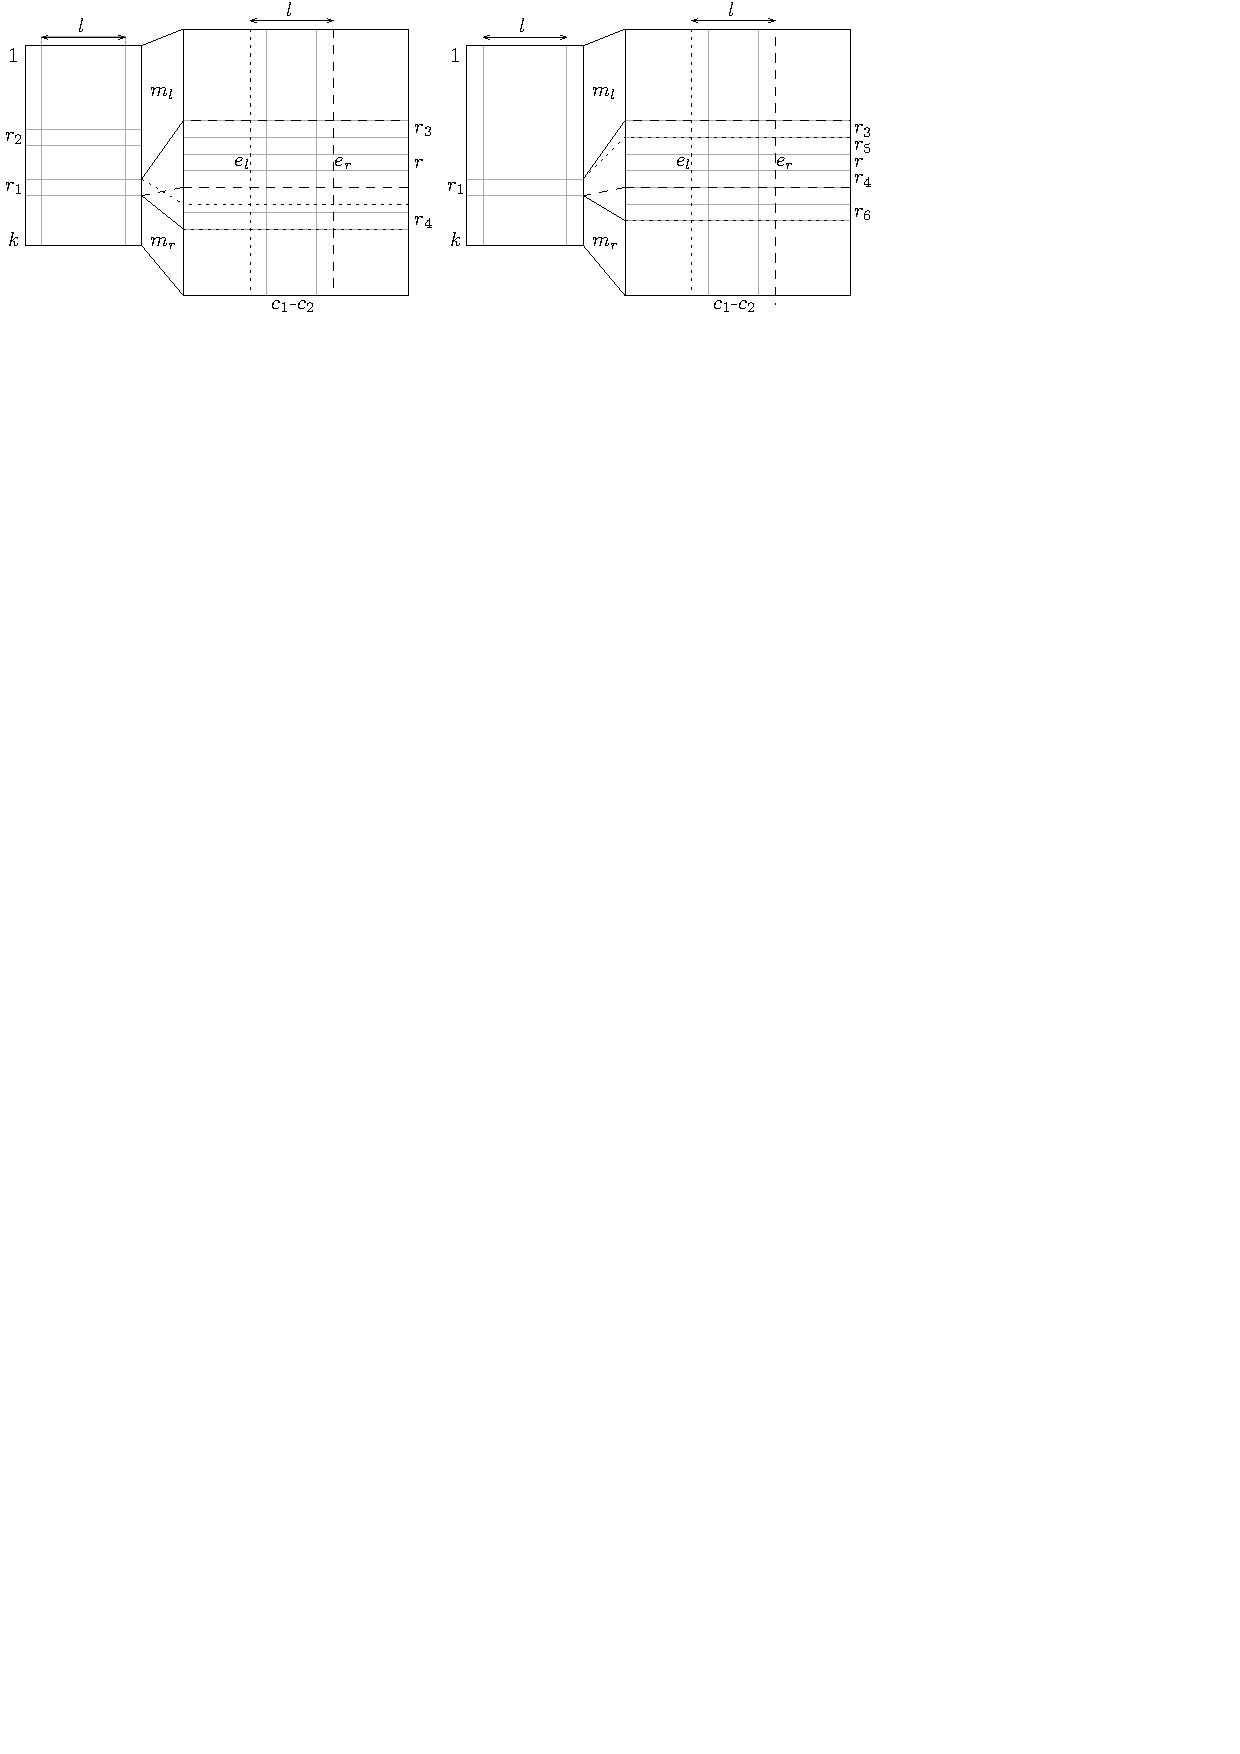
\includegraphics[width=\textwidth]{img/emptymid.pdf}
\caption{Dashed and dotted lines resembling two different mappings of a forbidden pattern, where two horizontal lines show the boundaries of the mapping of row~$r$ and the vertical lines show boundaries of the mapping of column~$c$.}
\label{fig:emptymid}
\end{figure}
\end{proof}

\begin{thm}
Let $P\in\{0,1\}^{k\times2}$ and for $l\geq1$ let $P^l\in\{0,1\}^{k\times l+2}$ be a pattern created from $P$ by adding a $l$ new empty columns in between the two columns of $P$. For all $M\in\Mat$ it holds $M\in Av(P^l)\Leftrightarrow$ there exists $N\in\{0,1\}^{m\times(n-l)}$ such that $N\in Av(P)$ is inclusion maximal and $M$ is a submatrix of elementwise OR of $N\oplus_h0^{m\times l},\ 0^{m\times 1}\oplus_hN\oplus_h0^{m\times(l-1)},\dots,\ 0^{m\times(l-1)}\oplus_hN\oplus_h0^{m\times1},\ 0^{m\times l}\oplus_hN$.
\end{thm}
\begin{proof}
\begin{itemize}
	\item[$\Rightarrow$] It suffices to only prove the statement for $M$ that is inclusion maximal. To do so, we use Lemma~\ref{lemma:maxmult}. It says that each row of $M$ contains either no one-entry or a single one-interval of length at least $l+1$. We consider $N$ to be created from $M$ by deleting the last $l$ one-entries on each row and excluding the last $l$ columns. Clearly, $M$ is equal to elementwise OR of $N\oplus_h0^{m\times l},\ 0^{m\times 1}\oplus_hN\oplus_h0^{m\times(l-1)},\dots,\ 0^{m\times(l-1)}\oplus_hN\oplus_h0^{m\times1},\ 0^{m\times l}\oplus_hN$. If $P\im N$ then each mapping of $P$ can be extended to a mapping of $P^l$ to $M$ by mapping each $P^l[i,1]$ to the same one-entry where $P[i,1]$ is mapped in $N\oplus_h0^{m\times l}$ and mapping each $P^l[j,l+2]$ to the same one-entry where $P[j,2]$ is mapped in $0^{m\times l}\oplus_hN$.
	\item[$\Leftarrow$] Let $M$ be equal to $N\oplus_h0^{m\times l}$ placed over $0^{m\times l}\oplus_hN$ with elementwise OR. It suffices to show that it belongs to $Av(P^l)$. For contradiction, assume it does not. Then there is mapping of $P^l$ to $M$ and we can assume that one-entries of the first column of $P^l$ are mapped to those one-entries of $M$ created from $N\oplus_h0^{m\times l}$. If there is such one-entry mapped to a one-entry of $M$ not created from $N\oplus_h0^{m\times l}$ we can take the first one-entry in the row instead. Symmetrically, all one-entries of the last column of $P^l$ are mapped to one-entries created from $0^{m\times1}\oplus_hN$. But then, then same one-entries of $N$ can be used to map $P$, which is a contradiction with $N\in Av(P)$.
\end{itemize}
\end{proof}

In Lemma~\ref{lemma:twocols} we proved half of the condition for a $k$ by 2 pattern to be bounded, here comes the second half.

\begin{obs}
Let $P\in\Pat$ and $M\in\Mat$ such that $\PnimM$. Let $zi=M[\{r_1\},[c_1,c_2]]$ be a zero-interval of $M$ usable for one-entry~$e=P[r,c]$. If we change a zero-entry of $zi$ and create a mapping of $P$ that uses the changed entry to map $e$, then no such mapping can map column~$c$ outside of columns $[c_1,c_2]$. 
\end{obs}
\begin{proof}
Since the changed entry is used to map $e$, clearly every mapping needs to use a column from $[c_1,c_2]$ to map column~$c$. If for contradiction after a change of a zero-entry there was a mapping using columns outside $[c_1,c_2]$ then it without loss of generality uses $c_1-1$ but since it bounds zero-interval~$zi$ it is a one-entry and this one-entry can be used in the mapping instead of the changed entry, which gives us a contradiction with $\PnimM$.
\end{proof}

\begin{lemma}
\label{lemma:twocols2}
Let $P\in\{0,1\}^{k\times 2}$ and $M\in\Mat$ be a maximal matrix avoiding $P$, then $M$ contains at most $2k^3+1$ one-intervals in each column.
\end{lemma}
\begin{proof}
Given an arbitrary maximal matrix~$M$ avoiding $P$ let us look at an arbitrary column~$c$. For contradiction, assume it has at least $2k^3+2$ one-intervals which also means there are at least $2k^3+1$ zero-intervals in between. Since $P$ has at most $2k$ one-entries, from the Pigeonhole principle there are $k^2$ (+1) zero-intervals $zi_1<zi_2<\dots<zi_{k^2}$ usable for the same one-entry~$e$ of $P$. Without loss of generality let $e=P[r,1]$.
\begin{itemize}
	\item $\forall i<r:\ P[i,2]=0$: If we take the mapping created by changing a zero-entry of $zi_k$ and to map $P[i,1]$ we use one-intervals above $zi_k$ we map the whole $P$, contradicting $\PnimM$.
	\item $P[r,2]=1$: Clearly, there is a one-entry next to each $zi_j$ and if we combine each such entry with a one-entry bounding each $zi_j$ we find a mapping of $\{1\}^{k^2\times2}$, contradicting $\PnimM$.
	\item $\exists i<r:\ P[i,2]=1$: If there are multiple such $i$, choose the biggest one, so that for all $i<j\leq r$ it holds $P[j,2]=0$. For all those $j$ it holds that $j$-th row of $P$ can be mapped to just one row of $M$. So first, if for any mapping $Map_1\dots Map_{k^2}$, created by changing a zero-entry of $zi_1\dots zi_{k^2}$ respectively to map $e$, is $i<l<r$ using two rows such that both have a one-entry in column~$c$, we can only use the first of them, shift the mapping off all following rows up to $r$ and find a mapping of $P$ to $M$. Therefore, we assume this is not the case and every mapping uses up to $r-i\leq k$ one-entries right above $zi_l$ it to map rows $[i,r-1]$.
	
		We combine the one-entry used to map $P[i,2]$ in mapping $Map_l$ with a one-entry bounding zero-interval $zi_l$. Since we have $k^2$ such mappings and each of them only goes through at most $k$ one-intervals to map $P[i,2]$ and therefore find a one-entry in a column~$c'>c$, we find at least $k$ distinct pairs and therefore a mapping of $\{1\}^{k\times2}$, contradicting $\PnimM$.
\end{itemize}
\end{proof}

\begin{cor}
Every $P\in\{0,1\}^{k\times 2}$ is bounded.
\end{cor}

\section{Pattern complexity}
We saw that for patterns having only two rows or columns we can indeed bound the number of one-intervals of maximal matrices avoiding them. On the other hand, already for a pattern of size $3\times3$ we show that there are maximal matrices with arbitrarily many one-intervals.

\begin{defn}
Let $\mathcal{P}$ be a class of patterns and for any $P\in\mathcal{P}$ let $e$ be a one-entry of $P$. We define the \emph{row-complexity of one-entry}~$e$ $r_\mathcal{P}(e)$ to be the supremum of the number of zero-intervals of a single row of any maximal matrix from $Av(\mathcal{P})$ that are usable for $e$. We say that $e$ is \emph{row-unbounded} in $\mathcal{P}$ if $r_\mathcal{P}(e)=\infty$ and \emph{row-bounded} otherwise. Symmetrically we define the \emph{column-complexity of one-entry}~$e$ $c_\mathcal{P}(e)$ to be the maximum number of zero-intervals of a single column of any maximal matrix from $Av(\mathcal{P})$ that are usable for $e$ and say $e$ is \emph{column-unbounded} if it is infinite and \emph{column-bounded} otherwise.
\end{defn}

\begin{defn}
Let $\mathcal{P}$ be a class of patterns. We define the \emph{row-complexity} of $\mathcal{P}$~$r_\mathcal{P}=sup\{r_\mathcal{P}(e)|e \text{ one-entry of } P\in\mathcal{P}\}$, the \emph{column-complexity} of $\mathcal{P}$~$c_\mathcal{P}=sup\{c_\mathcal{P}(e)|e \text{ one-entry of } P\in\mathcal{P}\}$ and the \emph{complexity} of $\mathcal{P}$~$comp_\mathcal{P}=sup\{r_\mathcal{P},c_\mathcal{P}\}$. We say $\mathcal{P}$ is \emph{unbounded} if $comp_\mathcal{P}=\infty$ and \emph{bounded} otherwise.
\end{defn}

The following observation follows directly the definition and we use it heavily throughout the chapter to break symmetries.

\begin{obs}
\label{obs:transposebounded}
For every $\mathcal{P},\ P\in\mathcal{P},\ P\in\Pat,\ r\in[k]$ and $c\in[l]$, if $P[r,c]$ is row-bounded in $Av(\mathcal{P})$ then $P^T[c,r]$ is column-bounded in $Av(\mathcal{P}^T)$. \qed
\end{obs}

\begin{thm}
\label{thm:manyints}
Let $P=\smm{ &\bullet& \\\bullet& & \\ & &\bullet}$. For every $n>1$ there is a maximal matrix $M$ avoiding $P$ as an interval minor having $n$ one-intervals ($P$ is unbounded).
\end{thm}
\begin{proof} Let $M$ be a $(2n-1)\times(2n-1)$ matrix described by the picture:
$$\smm{	\bullet& &\bullet& &\bullet&\cdots&\bullet& &\bullet& &\bullet\\
		 & & & & &\cdots& & &\bullet&\bullet&\bullet\\
		 & & & & &\cdots& & &\bullet&\bullet&\bullet\\
		 & & & & &\cdots&\bullet&\bullet&\bullet& & \\
		 & & & & &\cdots&\bullet&\bullet&\bullet& & \\
		\vdots&\vdots&\vdots&\vdots&\vdots&\vdots&\vdots&\vdots&\vdots&\vdots&\vdots\\
		 & &\bullet&\bullet&\bullet&\cdots& & & & & \\
		 & &\bullet&\bullet&\bullet&\cdots& & & & & \\
		\bullet&\bullet&\bullet& & &\cdots& & & & & \\
		\bullet&\bullet&\bullet& & &\cdots& & & & & \\
		 }$$
$\PnimM$ because we always need to map $P[2,1]$ and $P[3,3]$ to just one ``block'' of one-entries of $M$ which only leaves a zero-entry where we need to map $P[1,2]$.

When we change any zero-entry of the first row into a one-entry we get a matrix containing a minor of $\{1\}^{3\times3}$; therefore, containing $P$ as an interval minor. In case $M$ is not maximal, we can add some more one-entries to make it maximal but it will still contain a row with $n$ one-intervals.
\end{proof}

Not only $M$ is a maximal matrix avoiding $P$ but it also avoids any $P'\in\{0,1\}^{3\times3}$ such that $P\im P'$. Its rotations avoid rotations of $P$ and we can deduce that a big portion of patterns of size $3\times3$ are unbounded. Moreover, the result can be generalized also for bigger matrices. The pattern is so important that we call it $P_1$ for the rest of the chapter.

\begin{thm}
For every $P$ such that $P_1\im P$ and every $n>1$ there is a maximal matrix $M$ avoiding $P$ as an interval minor having $n$ one-intervals.
\end{thm}
\begin{proof}
First, assume there is a mapping of $P_1$ into $P\in\Pat$ that assigns a one-entry of the first row to $P_1[1,2]$, a one-entry of the first column to $P_1[2,1]$ and a one-entry of the last row and column to $P_1[3,3]$. Then, we can construct a similar matrix as we did in the proof of Theorem~\ref{thm:manyints} avoiding $P$ that after changing any zero-entry of the first row contains the whole $\{1\}^{k\times l}$.

Let $P$ be an arbitrary pattern containing $P_1$. Let $P[r_1,c_1],P[r_2,c_2]$ and $P[r_3,c_3]$ be one-entries that can be used to map $P_1[1,2],P_1[2,1]$ and $P_1[3,3]$ respectively. Then we take a submatrix $P':=P[[r_1,r_3],[c_2,c_3]]$. Such a pattern fulfills assumptions of the more restricted case stated at the beginning of the proof and we can find a maximal matrix $M'$ avoiding $P'$ having $n$ one-intervals. We construct $M$ from $M'$ by simply adding new rows and columns, all containing one-entries. We add $r_1-1$ rows in front of the first row and $k-r_3$ rows behind the last row. We also add $c_2-1$ columns in front of the first column and $l-c_3$ columns behind the last column. Constructed matrix $M$ avoids pattern $P$ as its submatrix $P'$ cannot be mapped to $M'$. At the same time, any change of a zero-entry of the $r_1$-th row of $M$ to a one-entry creates a copy of ${1}^{k\times l}$ so the changed matrix contains $P$. Constructed $M$ can be seen in Figure~\ref{fig:manyints}.

\begin{figure}[!ht]
\centering
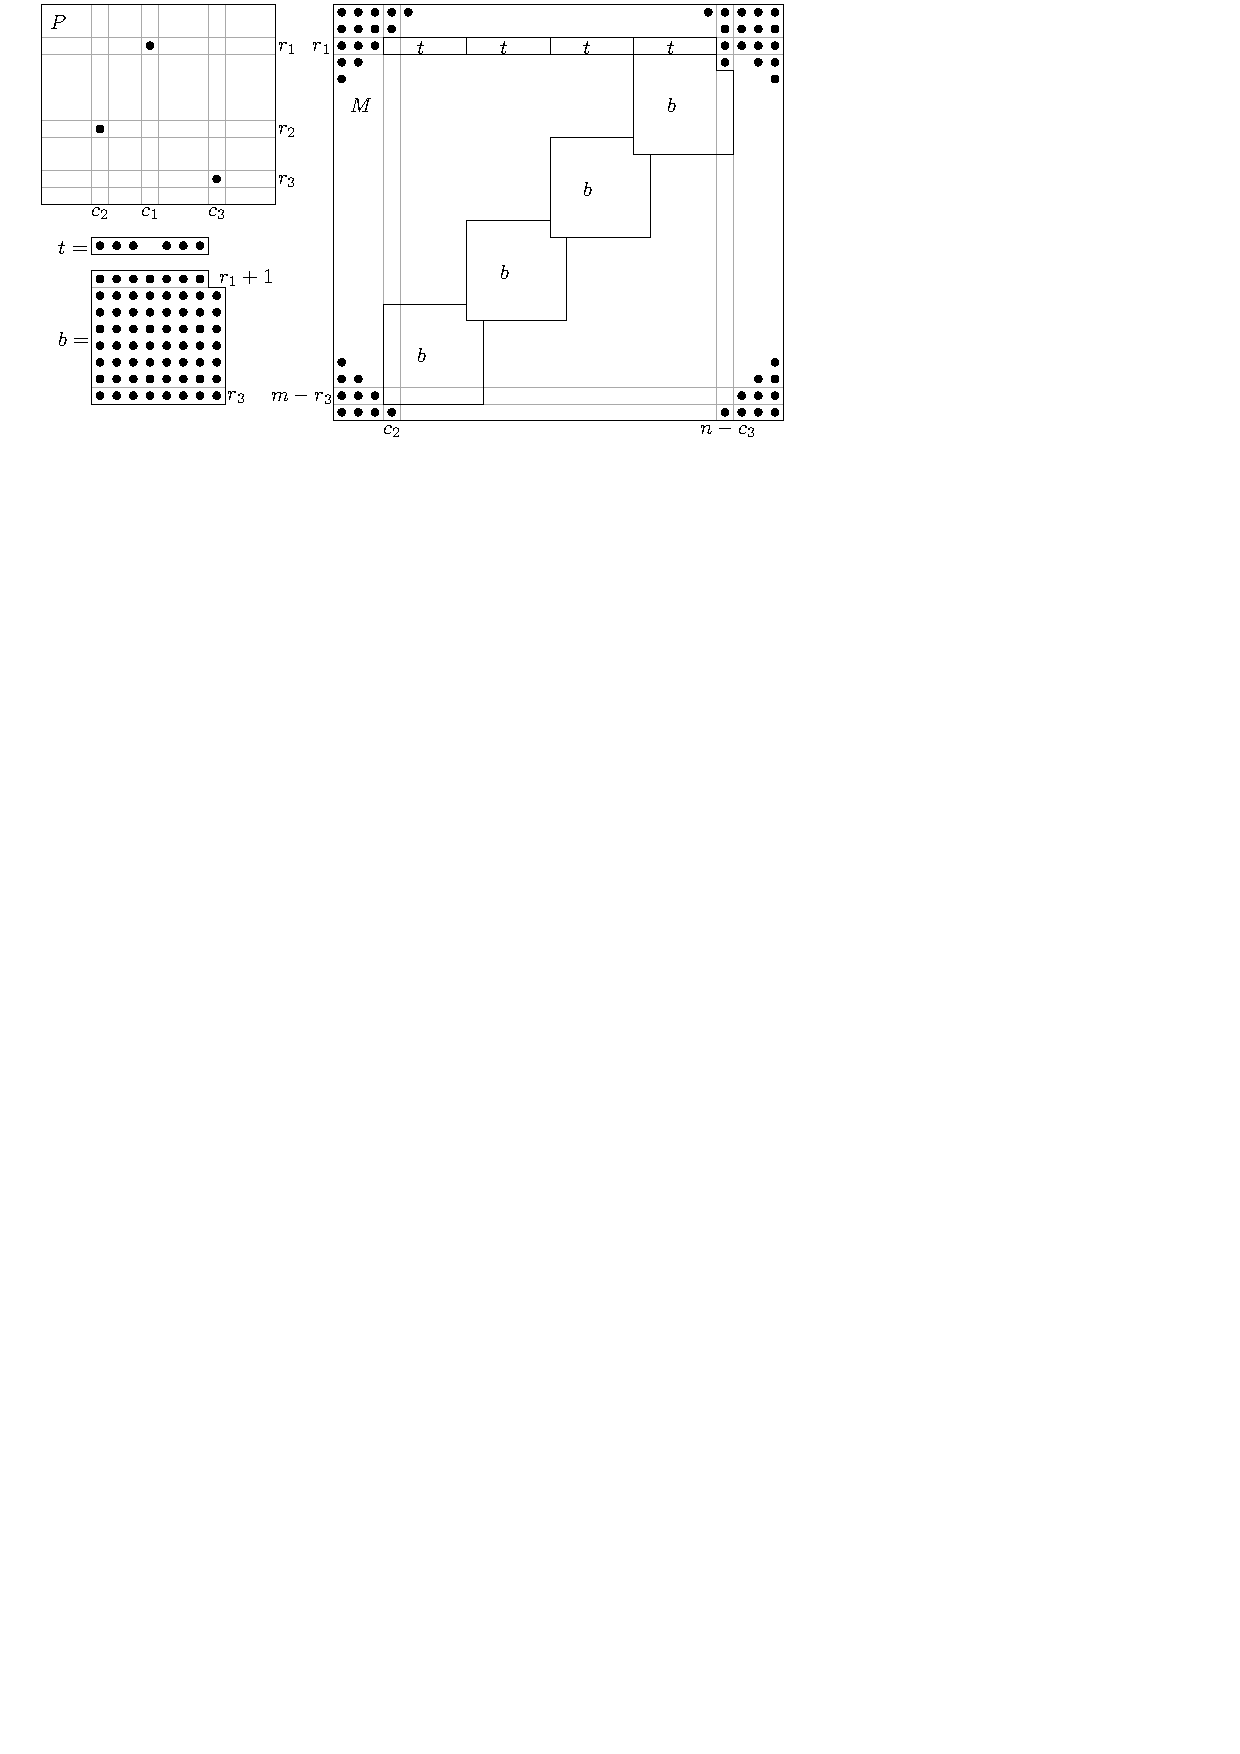
\includegraphics[width=120mm]{img/manyints.pdf}
\caption{Structure of a maximal matrix avoiding $P$ that has arbitrarily many one-intervals.}
\label{fig:manyints}
\end{figure}
\end{proof}

What makes it even more interesting is that any pattern avoiding all rotations of $P_1$ is already bounded. To prove that we need a few partial results.
\begin{thm}
\label{thm:boundedints}
Let $P$ be a pattern avoiding all rotations of $P_1$, then $P$:
\begin{enumerate}
	\item contains one non-empty line or
	\item contains two non-empty lines or
	\item contains three non-empty lines or
	\item avoids $\smm{\bullet& \\ &\bullet}$ or $\smm{ &\bullet\\\bullet& }$.
\end{enumerate}
\end{thm}
\begin{proof}
Assume $P$ has four one-entries that do not share any row or column. Then those one-entries induce a $4\times4$ permutation inside $P$ and because $P$ does not contain any rotation of $P_1$, the induced permutation is either $1234$ or $4321$. Without loss of generality, assume it is the first case and denote the one-entries by $e_1,e_2,e_3$ and $e_4$.

For contradiction with the statement, assume $P$ also contains $P'=\smm{\bullet& \\ &\bullet}$. Clearly, no one-entry from $e_1,e_2,e_3$ and $e_4$ can be part of any mapping of $P'$ because it would induce a mapping of a rotation of $P_1$.

Let $e_2=P[r_2,c_2]$ and $e_3=P[r_3,c_3]$. Submatrix~$P[[r_2],[c_2,l]]$ avoids $P'$; otherwise, together with $e_1$ it would give us a rotated copy of $P_1$. Symmetrically, $P[[r_3,k],[c_3]]$ does not contain $P'$. Also, $P[[r_3-1],[c_3-1]]$ and $P[[r_2+1,k],[c_2+1,l]]$ are empty; otherwise, they would together with $e_2$ and $e_3$ give us a rotation of $P_1$. Up to rotation, the only possible way to have $P'\im P$ is that $P'[1,1]$ lies in $P[[r_3-1],[c_2,c_3-1]]$ but then this entry together with $e_1$ and $e_3$ give us a rotation of $P_1$ which is a contradiction.
\end{proof}

Now comes the hard part. For each group of patterns, we need to prove they are bounded.

%%%%%%%%%%%%%%%%%%%%%%%%%%%%%%%%%%%%%%%%%%%%%%%%%% one non-empty line
\begin{lemma}
Let $P\in\Pat$ be a pattern having only one non-empty line. Then for every maximal matrix $M\in\Mat$ avoiding $P$ the number of one-intervals in each row and column is bounded by $k+l$. 
\end{lemma}
\begin{proof}
Without loss of generality let the non-empty line of $P$ be a row~$r$. Since $M$ is maximal, $M[[r-1],[n]]$ and $M[[m-r+1,m],[n]]$ contain no zero-entry and each of their rows contains just one interval of one-entries. If we look at any other row, it cannot contain $k$ one-entries, so the maximum number of one-intervals is $k-1$.

Let us look on an arbitrary column~$c$ of $M$. If there is at least one one-entry in $M[[r,m-r],c]$ then because $M$ is maximal, the whole column is made of one-entries. Otherwise, there are two intervals of one-entries -- $M[[r-1],c]$ and $M[[m-r,m],c]$.
\end{proof}

%%%%%%%%%%%%%%%%%%%%%%%%%%%%%%%%%%%%%%%%%%%%%%%%%% two non-empty lines
\begin{lemma}
Let $P\in\Pat$ be a pattern having two non-empty lines. Then for every maximal matrix $M\in\Mat$ avoiding $P$ the number of one-intervals in each row and column is bounded by $2k^3+2l^3+1$. 
\end{lemma}
\begin{proof}
First we assume the two non-empty lines of $P$ are rows $r_1<r_2$ (or symmetrically columns). From Observation~\ref{obs:emptyrows} and maximality of $M$ we have that $M[[r_1-1],[n]]$ and $M[[m-r_2+1,m],[n]]$ contain no zero-entry. Therefore, we may restrict ourselves to the case when $r_1=1$ and $r_2=k$. From Lemma~\ref{lemma:twocols2} we know that every maximal $N$ avoiding $P[\{r_1,r_2\},[n]]$ has at most $2k^3+1$ one-intervals in each row and at most $1$ one-interval in each column. From Theorem~\ref{thm:emptymiddle} we also know that for given $M$ there is a maximal $N$ avoiding $P[\{r_1,r_2\},[n]]$ such that $M$ is a submatrix of shifted and OR-ed copies of $N$. Since $M$ is maximal, it is equal to those shifted and OR-ed copies of $N$ and because the number of one-intervals of $N$ is bounded, so is the number of one-intervals of $M$.

Let the two non-empty lines of $P$ be row~$r$ and column~$c$. Because of symmetry, we only show the bound for rows. Let us take an arbitrary row of $M$ an look at its zero-intervals. For every one-entry~$e$ of the pattern except those in the $r$-th row, there is at most one zero-interval usable for $e$. For contradiction, assume there are two such zero-intervals $zi_1$ and $zi_2$. Let Figure~\ref{fig:twolines} illustrate the situation where dashed and dotted lines form mappings of the minor $P$ to $M$ when a zero-entry of $zi_1$ and $zi_2$ respectively is changed to a one-entry. When we take the outer two vertical and horizontal lines, we get a mapping of $P$ that can use an existing one-entry in between $zi_1$ and $zi_2$ to map $e$. This gives us a contradiction with $\PnimM$.

\begin{figure}[!ht]
\centering
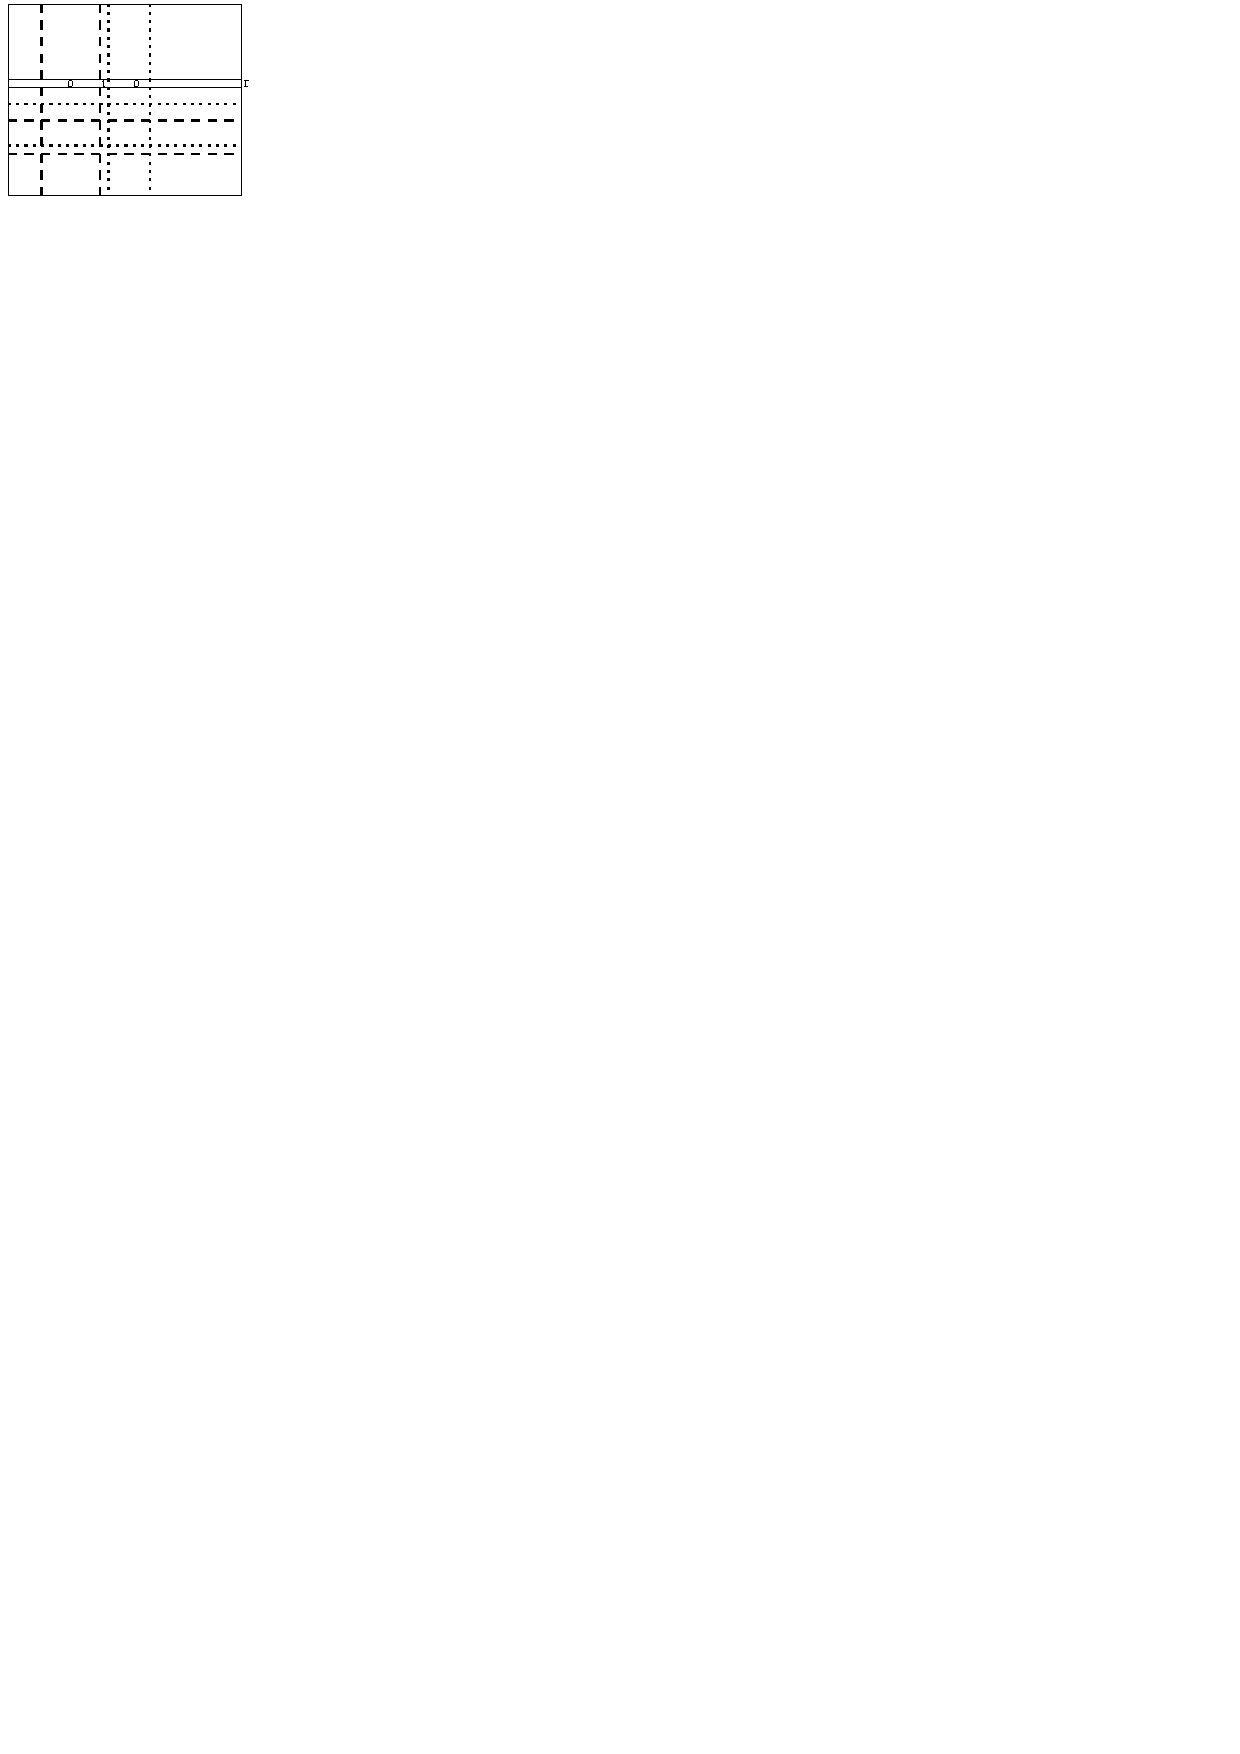
\includegraphics[width=70mm]{img/twolines.pdf}
\caption{Dashed and dotted lines resembling two different mappings of a forbidden pattern, where two horizontal lines show the boundaries of the mapping of row~$r$ and the vertical lines show boundaries of the mapping of column~$c$.}
\label{fig:twolines}
\end{figure}

For a one-entry $e=P[r,c']$, if $c'\leq c$ then there must be less than $c'$ one-entries before any zero-intervals usable for $e$; otherwise, we could map $P[r,[1,c']]$ just to the single row of $M$. It follows that $e$ is row-bounded. Symmetrically, the same holds in case $c'>c$. 
\end{proof}

To make the analysis of the last two groups of patterns easier, we introduce three helpful lemmata.

%%%%%%%%%%%%%%%%%%%%%%%%%%%%%%%%%%%%%%%%%%%%%% Lemma H
\begin{lemma}
\label{lemma:H}
Let $P\in\Pat$ be a pattern structured like one of the matrices in Figure~\ref{fig:lemmaH}. Then every one-entry in $P[\{r_2\},[c_1,c_2]]$ is row-bounded.

\begin{figure}[!ht]
\centering
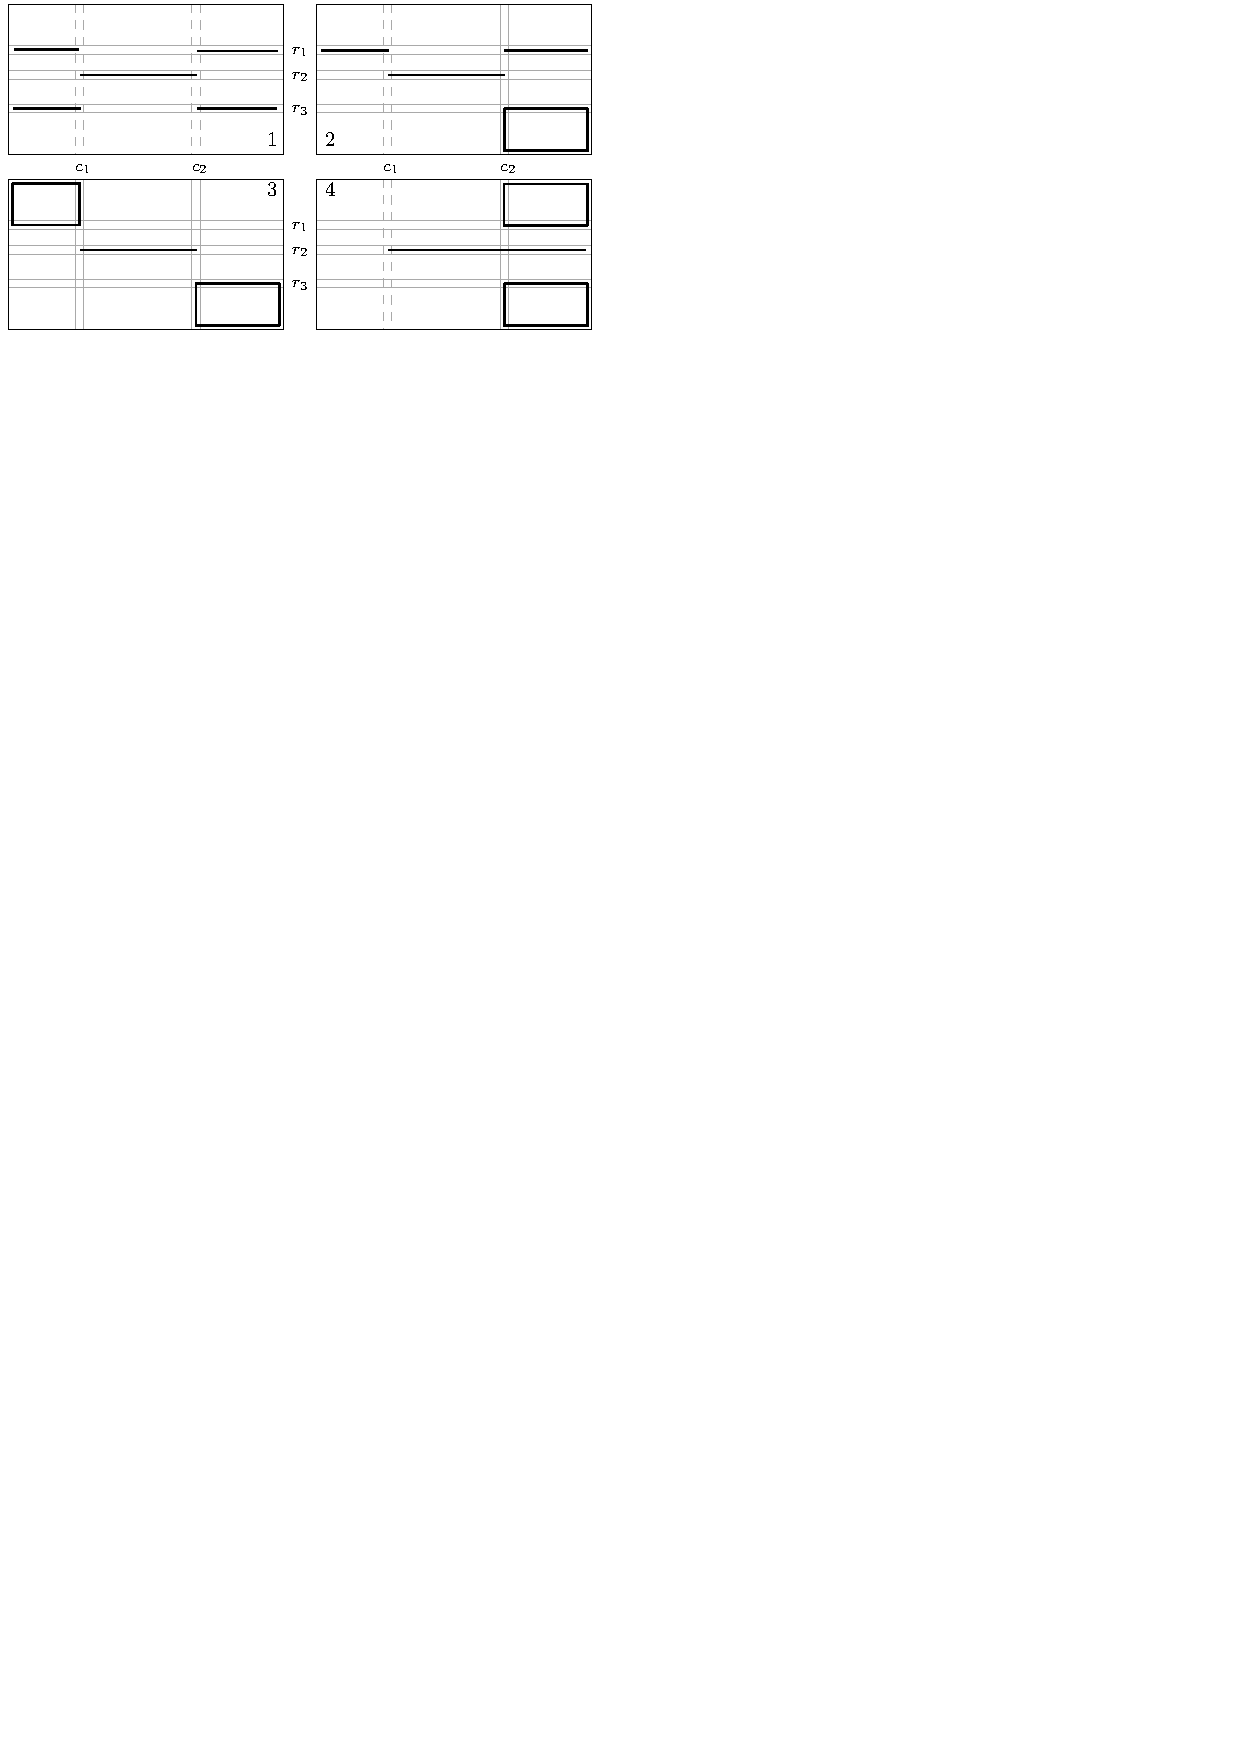
\includegraphics[width=\textwidth]{img/lemmaH.pdf}
\caption{Patterns for which one-entries in row~$r_2$ and columns $c_1$ to $c_2$ are row-bounded. One-entries may only be in the areas enclosed by bold lines.}
\label{fig:lemmaH}
\end{figure}
\end{lemma}
\begin{proof}
Let $P$ be the first described pattern and let $k'=c_2-c_1$. We show that for each one-entry $e$ from row~$r_2$ and every $M$ maximal matrix avoiding $P$ there is at most $k'$ zero-intervals for which it is usable. For contradiction assume there is a row~$r$ with $k'+1$ zero-intervals usable for $e$. It follows that there are at least $k'$ one-entries in between two most distant zero-intervals $z_1$ and $z_2$. Therefore, the whole row~$r_2$ can be mapped just to $r$. Since changing a zero-entry of $z_1$ to a one-entry to which $e$ can be mapped creates a partitioning of $M$ where all one-entries from columns $1$ to $c_1$ are mapped to columns up to $z_1$ and similarly all one-entries from columns $c_2$ to $l$ can be mapped to columns from and past $z_2$, we can simply map empty rows from $r_1+1$ to $r_3-1$ around row $r$ and use the rest to map rows $r_1$ and $r_2$. Described partitioning gives us $\PimM$ and a contradiction. We can see the partitioning in Figure~\ref{fig:lemmaH1}.
\begin{figure}[!ht]
\centering
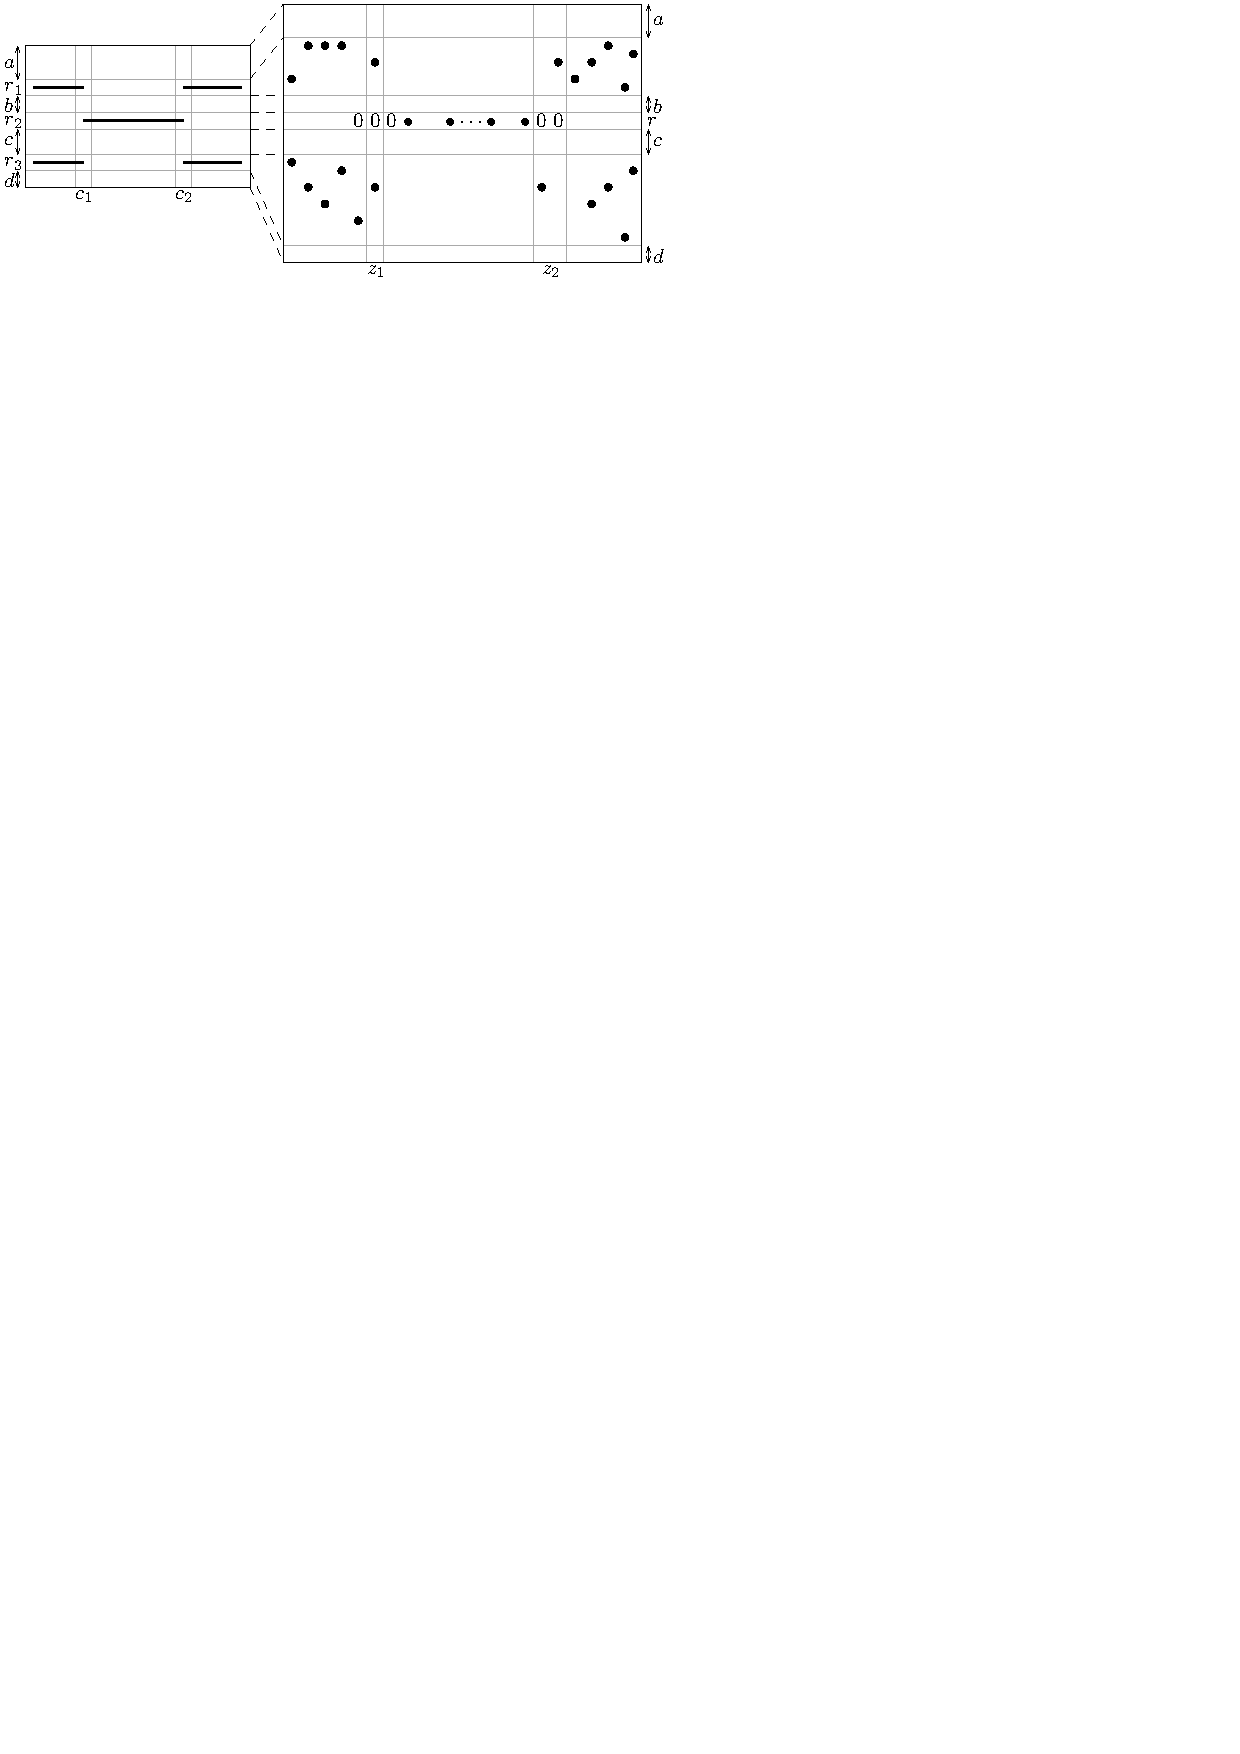
\includegraphics[width=\textwidth]{img/lemmaH1.pdf}
\caption{Mapping of a pattern into a matrix only using one line to map an empty line of the pattern and only using one line to map row~$r_2$.}
\label{fig:lemmaH1}
\end{figure}

Proofs of cases two and three are similar to the first one and we skip them.

Let us look on the fourth case. For $i$-th one-entry in row~$r_2$ (ordered from left to right and only considering those in columns $c_1$ to $c_2$) no zero-interval of a maximal matrix avoiding the pattern cannot have $i$ one-entries to the left of it and so each such one-entry is bounded by $i\geq l$.

It is important to realize we could not have used the same proof we used for the first three cases also for the fourth case, because we can never rely on the fact a mapping of $P$ only uses one row of $M$ to map row~$r_2$. This is because in the fourth case, unlike the first three, there are also potential one-entries in $P[\{r_2\},[c_2,l]]$.
\end{proof}

%%%%%%%%%%%%%%%%%%%%%%%%%%%%%%%%%%%%%%%%%%%% Lemma I
\begin{lemma}
\label{lemma:I}
Let $P\in\Pat$ be a pattern structured like one of the matrices in Figure~\ref{fig:lemmaI}. Then every one-entry in $P[[r_1+1,r_2-1],\{c\}]$ is row-bounded.

\begin{figure}[!ht]
\centering
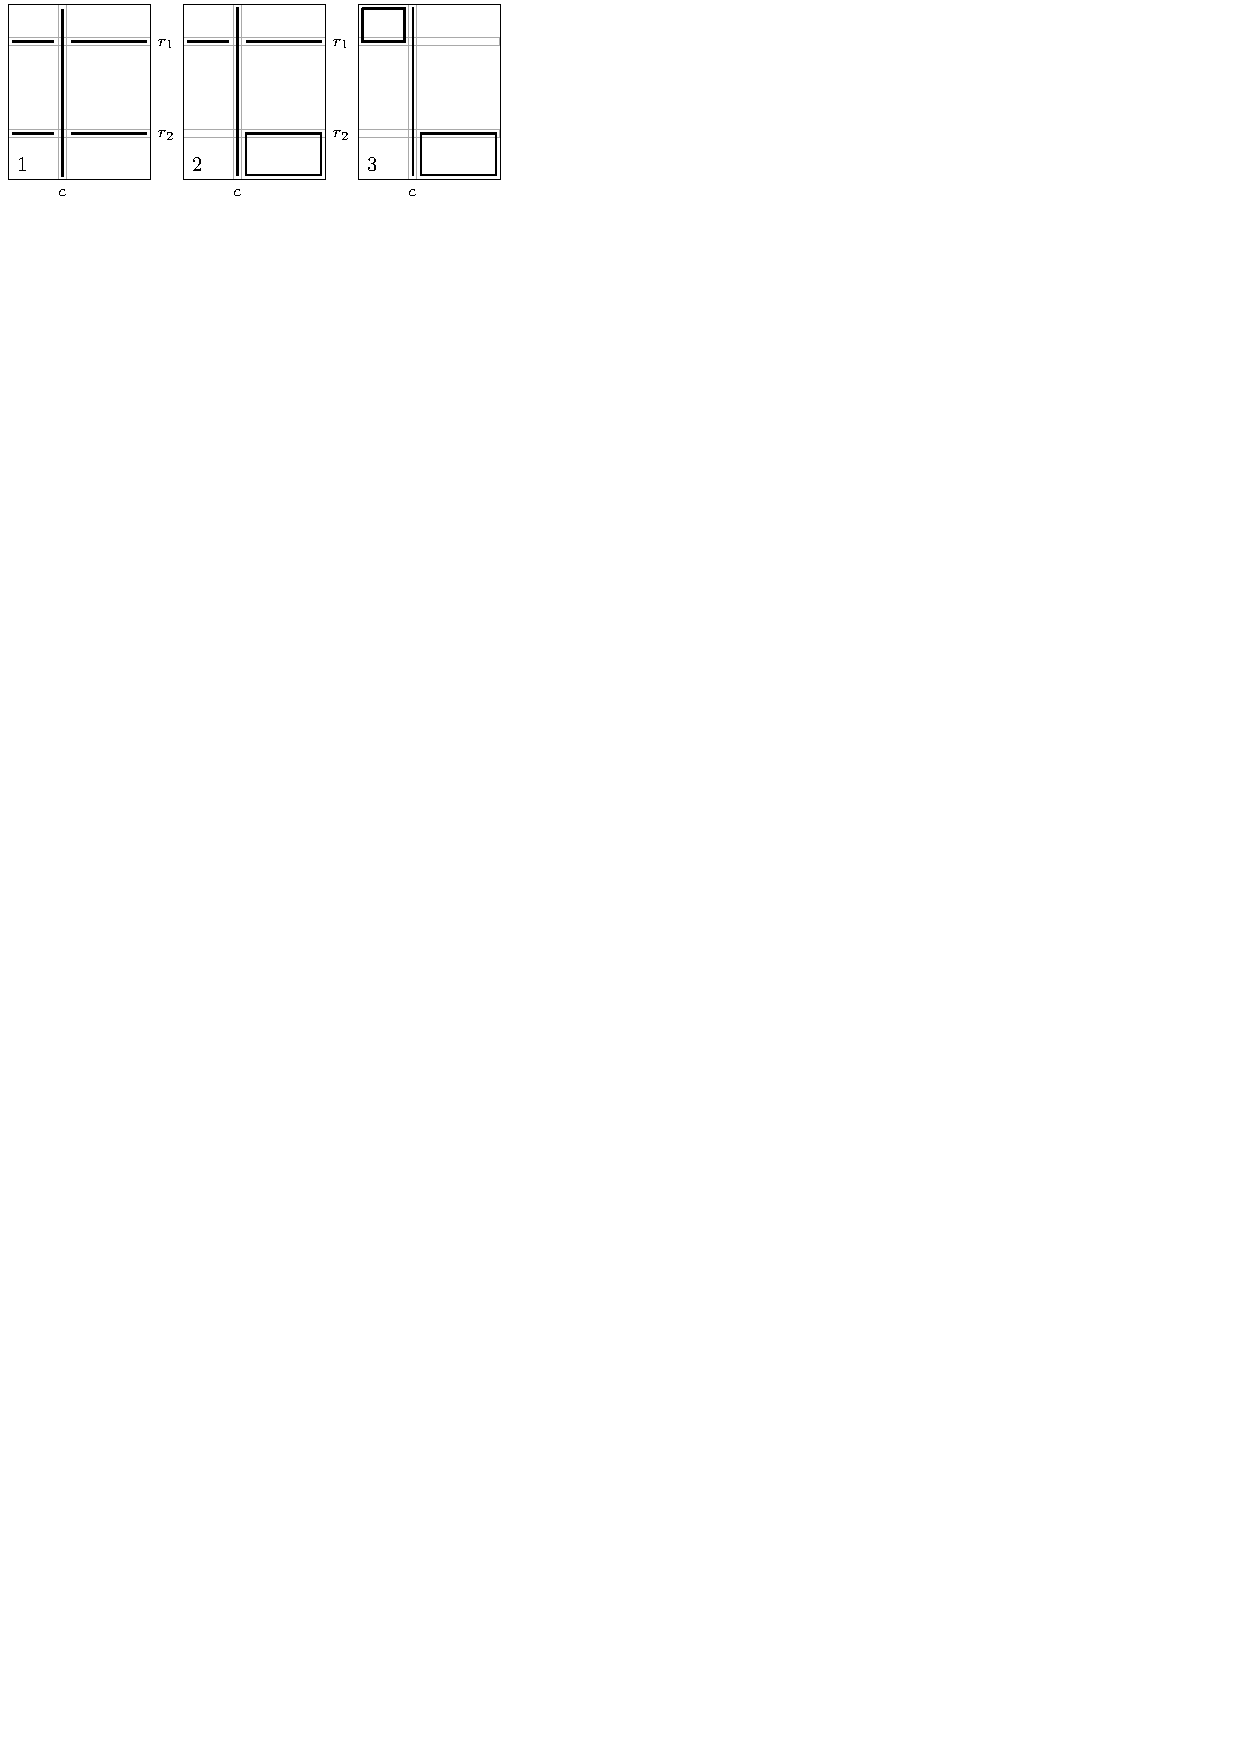
\includegraphics[width=120mm]{img/lemmaI.pdf}
\caption{Patterns for which one-entries in column~$c$ are row-bounded. One-entries may only be in the areas enclosed by bold lines.}
\label{fig:lemmaI}
\end{figure}
\end{lemma}
\begin{proof}
Let $P$ be the first described pattern. We show that for each one-entry $e$ from row~$r_2$ and every $M$ maximal matrix avoiding $P$ there is at most one zero-interval for which it is usable. For contradiction assume there is a row~$r$ with two zero-intervals $z_1$ and $z_2$ usable for $e$. Look at Figure~\ref{fig:lemmaI1} and let the dashed partitioning be a mapping of $P$ to $M$ when a zero-entry of $z_1$ is changed to a one-entry used to map $e$ and let the dotted partitioning be a mapping of $P$ to $M$ when a zero-entry of $z_2$ is changed to a one-entry used to map $e$. If we map column $c$ to where it is mapped in both mappings together and map rows $r_1$ and $r_2$ as suggested in the picture, we get a partitioning of $P$ inside $M$ and so a contradiction with $\PnimM$.

\begin{figure}[!ht]
\centering
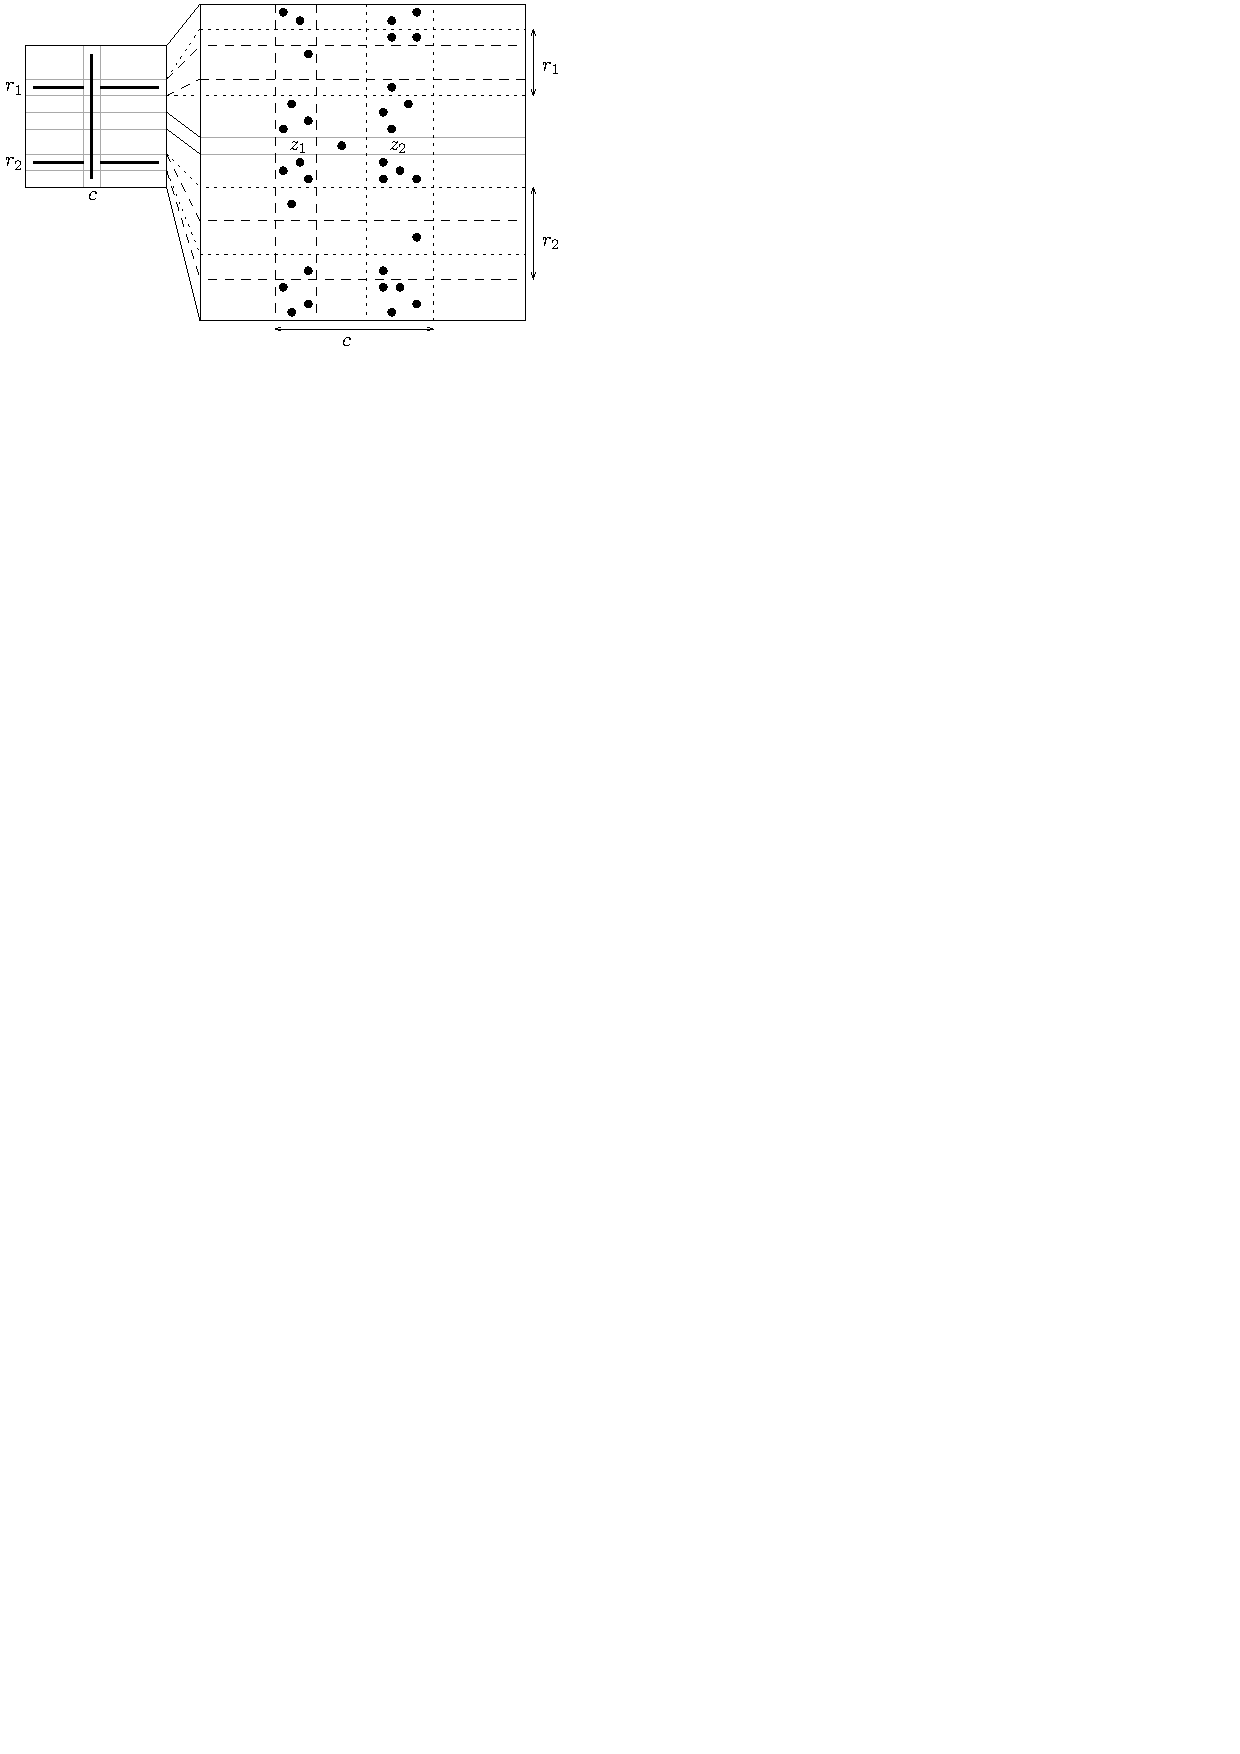
\includegraphics[width=100mm]{img/lemmaI1.pdf}
\caption{}
\label{fig:lemmaI1}
\end{figure}

Proofs of cases two and three are similar to the first one and we skip them.
\end{proof}

\begin{thm}
Let $P$ be a pattern and $e$ be any of its one-entries. Then $e$ is row-unbounded if and only if it can be used to map:
\begin{itemize}
\item $P_1[1,2]$ in any mapping of $P_1$ to $P$ or
\item $P_2[1,2]$ in any mapping of $P_2$ to $P$ or
\item $P_3[3,2]$ in any mapping of $P_3$ to $P$ or
\item $P_4[3,2]$ in any mapping of $P_4$ to $P$.
\end{itemize}
\end{thm}
\begin{proof}
\begin{itemize}
\item[$\Leftarrow$] If $e$ is contained in any of those mappings, we can use the construction from Theorem~\ref{thm:manyints} to show that $e$ is row-unbounded.
\item[$\Rightarrow$] TODO
\end{itemize}
\end{proof}

%%%%%%%%%%%%%%%%%%%%%%%%%%%%%%%%%%%%%%%%%%%%%% First non-empty column bounded
\begin{lemma}
\label{lemma:First}
Let $P$ be a pattern and $c$ be its first non-empty column. Then every one-entry from $c$ is row-bounded.
\end{lemma}
\begin{proof}
The result follows immediately from the fourth case of Lemma~\ref{lemma:H}.
\end{proof}

%%%%%%%%%%%%%%%%%%%%%%%%%%%%%%%%%%%%%%%%%% walking patterns
\begin{lemma}
\label{lemma:walkpat}
Let $P\in\Pat$ be a pattern avoiding $\smm{ &\bullet\\\bullet& }$ (or $\smm{\bullet& \\ &\bullet}$). Then for every maximal matrix $M\in\Mat$ avoiding $P$ the number of one-intervals in each row and column is bounded.
\end{lemma}
\begin{proof}
From Theorem~\ref{thm:walking} we know that $P$ is a walking pattern. Every one-entry of $P$ satisfies either conditions of the third case of Lemma~\ref{lemma:H} or it satisfies conditions of the third case of Lemma~\ref{lemma:I} and therefore is row-bounded. To prove it is also column-bounded, we use Observation~\ref{obs:transposebounded}.
\end{proof}

%%%%%%%%%%%%%%%%%%%%%%%%%%%%%%%%%%%%%%%%%%% three non-empty lines - it is super long
\begin{lemma}
Let $P\in\Pat$ be a pattern having three non-empty lines and avoiding all rotations of $P_1$. Then for every maximal matrix $M\in\Mat$ avoiding $P$ the number of one-intervals in each row and column is bounded. 
\end{lemma}
\begin{proof}
First of all, if $P$ avoids $\smm{ &\bullet\\\bullet& }$ or $\smm{\bullet& \\ &\bullet}$ we can use Lemma~\ref{lemma:walkpat}. Therefore, we assume it contains both.

Let us prove that each pattern having one-entries in three rows is bounded. If all one-entries are in up to two columns then we are again done. Therefore, $P$ has one-entries in at least three columns and it contains a three by three permutation matrix as a submatrix. Since rotations of $P_1$ are avoided, only feasible permutations are 123 and 321 and without loss of generality we assume the first case. In Figure~\ref{fig:threelines} we see the structure of each such pattern. Capital letters stand for one-entries of the permutation, letters $a-f$ stand each for a potential one-entry and greek letters stand each for a potential sequence of one-entries and zero-entries. Everything else is zero. Not all one-entries can be present at the same time, because that would create a mapping of $P_1$ or its rotation but we also need to find $\smm{\bullet& \\ &\bullet}$. The following analysis only uses hereditary arguments. This means that if we prove $P$ is bounded, we also prove that each submatrix of $P$ is bounded. With this in mind, we restrict ourselves to maximal patterns.
\begin{itemize}
	\item $\gamma$ contains a one-entry $\Rightarrow f=0\Rightarrow$ because $\smm{\bullet& \\ &\bullet}$ needs to be there it holds $a=1\Rightarrow\alpha=0$
		\begin{itemize}
			\item $d=1\Rightarrow b=0,\ \beta=0,\ e=0,\ c=?$:\\
				Lemma~\ref{lemma:H} (case 4): one-entries in $c,C,\gamma$ are row-bounded.\\
				Lemma~\ref{lemma:First}: $a$ and $A$ are row-bounded.\\
				Lemma~\ref{lemma:I} (case 1): $d$ and $B$ are row-bounded.\\
				
				Lemma~\ref{lemma:First}: all one-entries except for $B$ are column-bounded.\\
				Lemma~\ref{lemma:H} (case 1): $B$ is column-bounded.
			\item $d=0$
				\begin{itemize}
					\item $c=1\Rightarrow\beta=0,\ e=0,\ b=?$:\\
						Lemma~\ref{lemma:H} (case 4): one-entries in $c,C,\gamma$ are row-bounded.\\
						Lemma~\ref{lemma:First}: $a,b,A$ are row-bounded.\\
						Lemma~\ref{lemma:H} (case 1): $B$ is row-bounded.\\
						
						Lemma~\ref{lemma:First}: one-entries in the first and the third non-empty rows are column-bounded.\\
						Lemma~\ref{lemma:H} (case 2): $b,B$ are column-bounded.
					\item $c=0\Rightarrow$ in the maximal case $b=1,\ e=1,\ \gamma$ contains a one-entry:\\
						Lemma~\ref{lemma:H} (case 4): one-entries in $c,C,\gamma$ are row-bounded.\\
						Lemma~\ref{lemma:First}: one-entries in the first non-empty column are row-bounded.\\
						Lemma~\ref{lemma:H} (case 1): one-entries in the middle non-empty row are row-bounded.\\
						
						Lemma~\ref{lemma:First}: one-entries in the first and the third non-empty rows are column-bounded.\\
						Lemma~\ref{lemma:I} (case 2): one-entries in the middle non-empty row are column-bounded.
				\end{itemize}
		\end{itemize}
	\item $\gamma=0$
		\begin{itemize}
			\item $\alpha$ contains a one-entry $\Rightarrow a=0,\ b=0$:\\
				Every such pattern has already been dealt with as we can rotate it by 180 degrees, map $A$ and $\alpha$ to $\gamma$, map $d$ to $C$ and so on.
			\item $\alpha=0$:\\
				Without loss of generality, we can assume that $a=1$, because there needs to be $\smm{ &\bullet\\\bullet& }$ and if we set $a=0$, it must hold $f=1$ and then we can just rotate the pattern by 180 degrees and get the case $a=1$.
				\begin{itemize}
					\item $d=1\Rightarrow b=0,\ e=0,\ \beta=0,\ c=?,\ f=?$:\\
						Lemma~\ref{lemma:First}: $a,f,A$ and $C$ are row-bounded.\\
						Lemma~\ref{lemma:I} (case 1): $c,d$ and $B$ are row-bounded.\\
						
						Lemma~\ref{lemma:First}: one-entries in the first and third non-empty rows are column-bounded.\\
						Lemma~\ref{lemma:H} (case 1): $B$ is column-bounded.
					\item $d=0$
						\begin{itemize}
							\item $e=1\Rightarrow c=0,\ b=?,\ f=?$:\\
								Since $\alpha=0$ it follows that if there is a one-entry in $\beta$ only if it can be in $e$.
								
								Lemma~\ref{lemma:First}: $a,f,A$ and $C$ are row-bounded.\\
								Lemma~\ref{lemma:H} (case 1): one-entries in $b,e,B$ and $\beta$ are row-bounded. \\
								
								Lemma~\ref{lemma:First}: $a,f,A$ and $C$ are column-bounded.\\
								Lemma~\ref{lemma:I} (case 1): one-entries in $b,e,B$ and $\beta$ are column-bounded.
							\item $e=0$:\\
								We can assume $c=1$ as else $e$ can be 1 and we have already dealt with that case. We can also assume $b=1$ since otherwise, we would have a submatrix of the case dealt with when $d=1$:\\
								Lemma~\ref{lemma:First}: $a,b$ and $A$ are row-bounded.\\
								Lemma~\ref{lemma:H} (case 4): $c$ and $C$ are row-bounded.\\
								Lemma~\ref{lemma:H} (case 1): $B$ is row-bounded.\\
										
								Because the pattern is symmetric, it is also column-bounded.
						\end{itemize}
				\end{itemize}
		\end{itemize}
\end{itemize}
The same analysis also proves that if the pattern with the same restrictions only has three non-empty columns then it is bounded.
\begin{figure}[!ht]
	\centering
	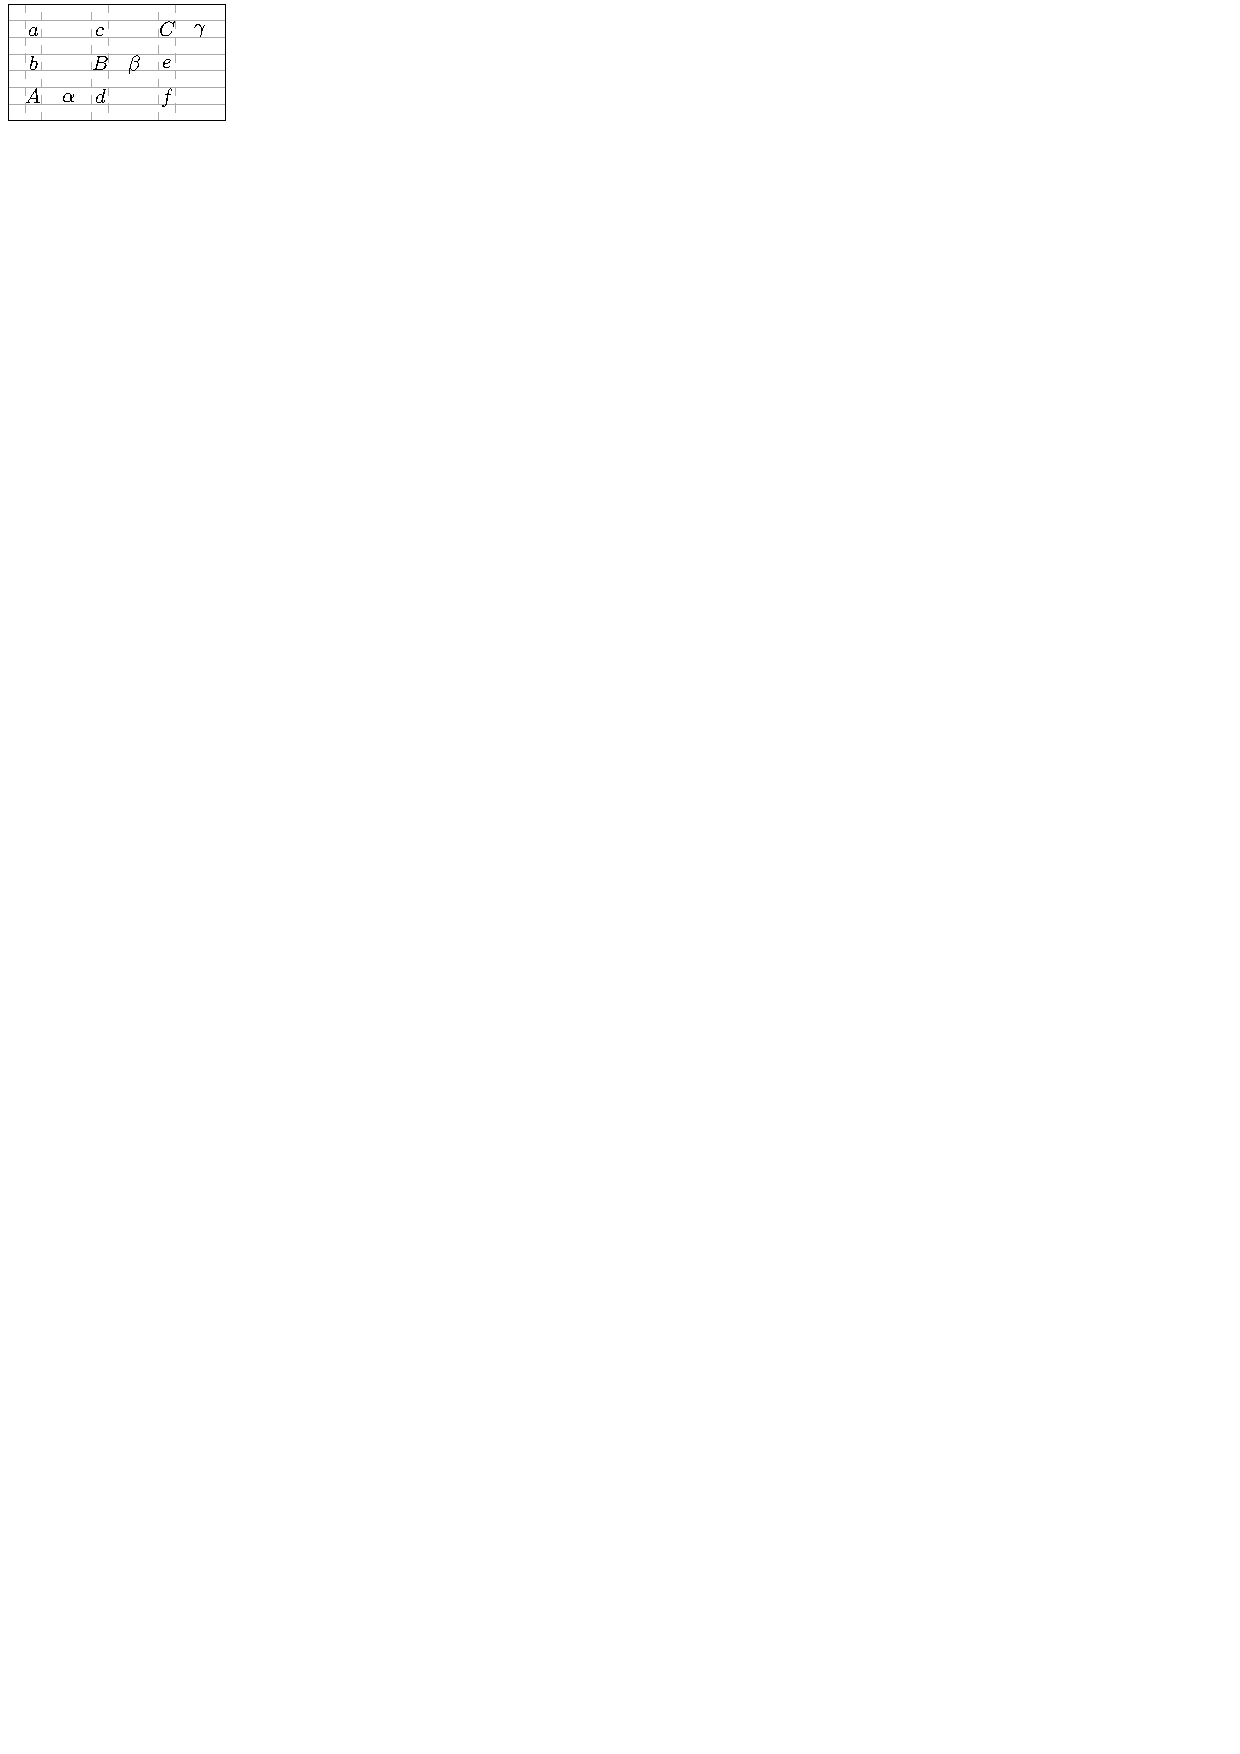
\includegraphics[width=70mm]{img/threelines.pdf}
	\caption{Structure of a pattern only having three non-empty rows and avoiding all rotations of $P_1$.}
	\label{fig:threelines}
\end{figure}

Let us now look at the case where all one-entries of the pattern are in either one of two rows $r_1,r_2$ or in column~$c_1$. Without loss of generality, we again assume permutation 123 is present and we distinguish three cases. Consider Figure~\ref{fig:twoplusone}:
\begin{itemize}
\item $C$ lies in column~$c_1$
	\begin{itemize}
		\item $a=1\Rightarrow b=0,\ \alpha=0$ and everything else can be one:\\
			Lemma~\ref{lemma:H} (case 2): one-entries in $a,c,B$ and $\beta$ are row-bounded.\\
			Lemma~\ref{lemma:First}: all other one-entries are row-bounded.\\
			
			Lemma~\ref{lemma:H} (case 4): one-entries in $c,C$ and $\gamma$ are column-bounded.\\
			Lemma~\ref{lemma:I} (case 1): one-entries in $a,c,B$ and $\beta$ are column-bounded.\\
			Lemma~\ref{lemma:First}: $d$ and $A$ are column-bounded.
		\item $a=0$ and everything else can be one:\\
			Lemma~\ref{lemma:H} (case 4): one-entries in $b,A$ and $\alpha$ are row-bounded.\\
			Lemma~\ref{lemma:H} (case 2): one-entries in $c,B$ and $\beta$ are row-bounded.\\
			Lemma~\ref{lemma:First}: one-entries in $c,d,C$ and $\gamma$ are row-bounded.\\
			
			Lemma~\ref{lemma:H} (case 4): one-entries in $c,C$ and $\gamma$ are column-bounded.\\
			Lemma~\ref{lemma:I} (case 2): one-entries in $c,B$ and $\beta$ are column-bounded.\\
			Lemma~\ref{lemma:First}: one-entries in $b,d,A$ and $\alpha$ are column-bounded.			
	\end{itemize}
\item $B$ lies in column~$c_1$
	\begin{itemize}
		\item $a=1\Rightarrow\alpha=0$
			\begin{itemize}
				\item $d=1\Rightarrow\gamma=0$:\\
					Lemma~\ref{lemma:I} (case 1): all one-entries in column $c_1$ are row-bounded.\\
					Lemma~\ref{lemma:First}: all other one-entries are row-bounded.\\
					
					Lemma~\ref{lemma:H} (case 1): all one-entries in column $c_1$ are column-bounded.\\
					Lemma~\ref{lemma:First}: all other one-entries are column-bounded.
				\item $d=0$:\\
					Lemma~\ref{lemma:I} (case 1): all one-entries in column $c_1$ are row-bounded.\\
					Lemma~\ref{lemma:First}: $a$ and $A$ are row-bounded.\\
					Lemma~\ref{lemma:H} (case 4): one-entries in $C$ and $\gamma$ are row-bounded.\\
					
					Lemma~\ref{lemma:H} (case 1): all one-entries in column $c_1$ are column-bounded.\\
					Lemma~\ref{lemma:First}: all other one-entries are column-bounded.
			\end{itemize}
		\item $a=0$
			\begin{itemize}
				\item $d=1\Rightarrow\gamma=0$:\\
					Lemma~\ref{lemma:I} (case 1): all one-entries in column $c_1$ are row-bounded.\\
					Lemma~\ref{lemma:First}: $d$ and $C$ are row-bounded.\\
					Lemma~\ref{lemma:H} (case 4): one-entries in $A$ and $\alpha$ are row-bounded.\\
					
					Lemma~\ref{lemma:H} (case 1): all one-entries in column $c_1$ are column-bounded.\\
					Lemma~\ref{lemma:First}: all other one-entries are column-bounded.
				\item $d=0$:\\
					Lemma~\ref{lemma:I} (case 1): all one-entries in column $c_1$ are row-bounded.\\
					Lemma~\ref{lemma:H} (case 4): one-entries in $A,C,\alpha$ and $\gamma$ are row-bounded.\\
					
					Lemma~\ref{lemma:H} (case 1): all one-entries in column $c_1$ are column-bounded.\\
					Lemma~\ref{lemma:First}: all other one-entries are column-bounded.
			\end{itemize}
	\end{itemize}
\item $A$ lies in column~$c_1$:\\
	This is the first situation rotated by 180 degrees.
\end{itemize}
The same analysis also proves that if one-entries of a pattern with the same restrictions are in one row or two columns then the pattern is bounded.
\begin{figure}[!ht]
	\centering
	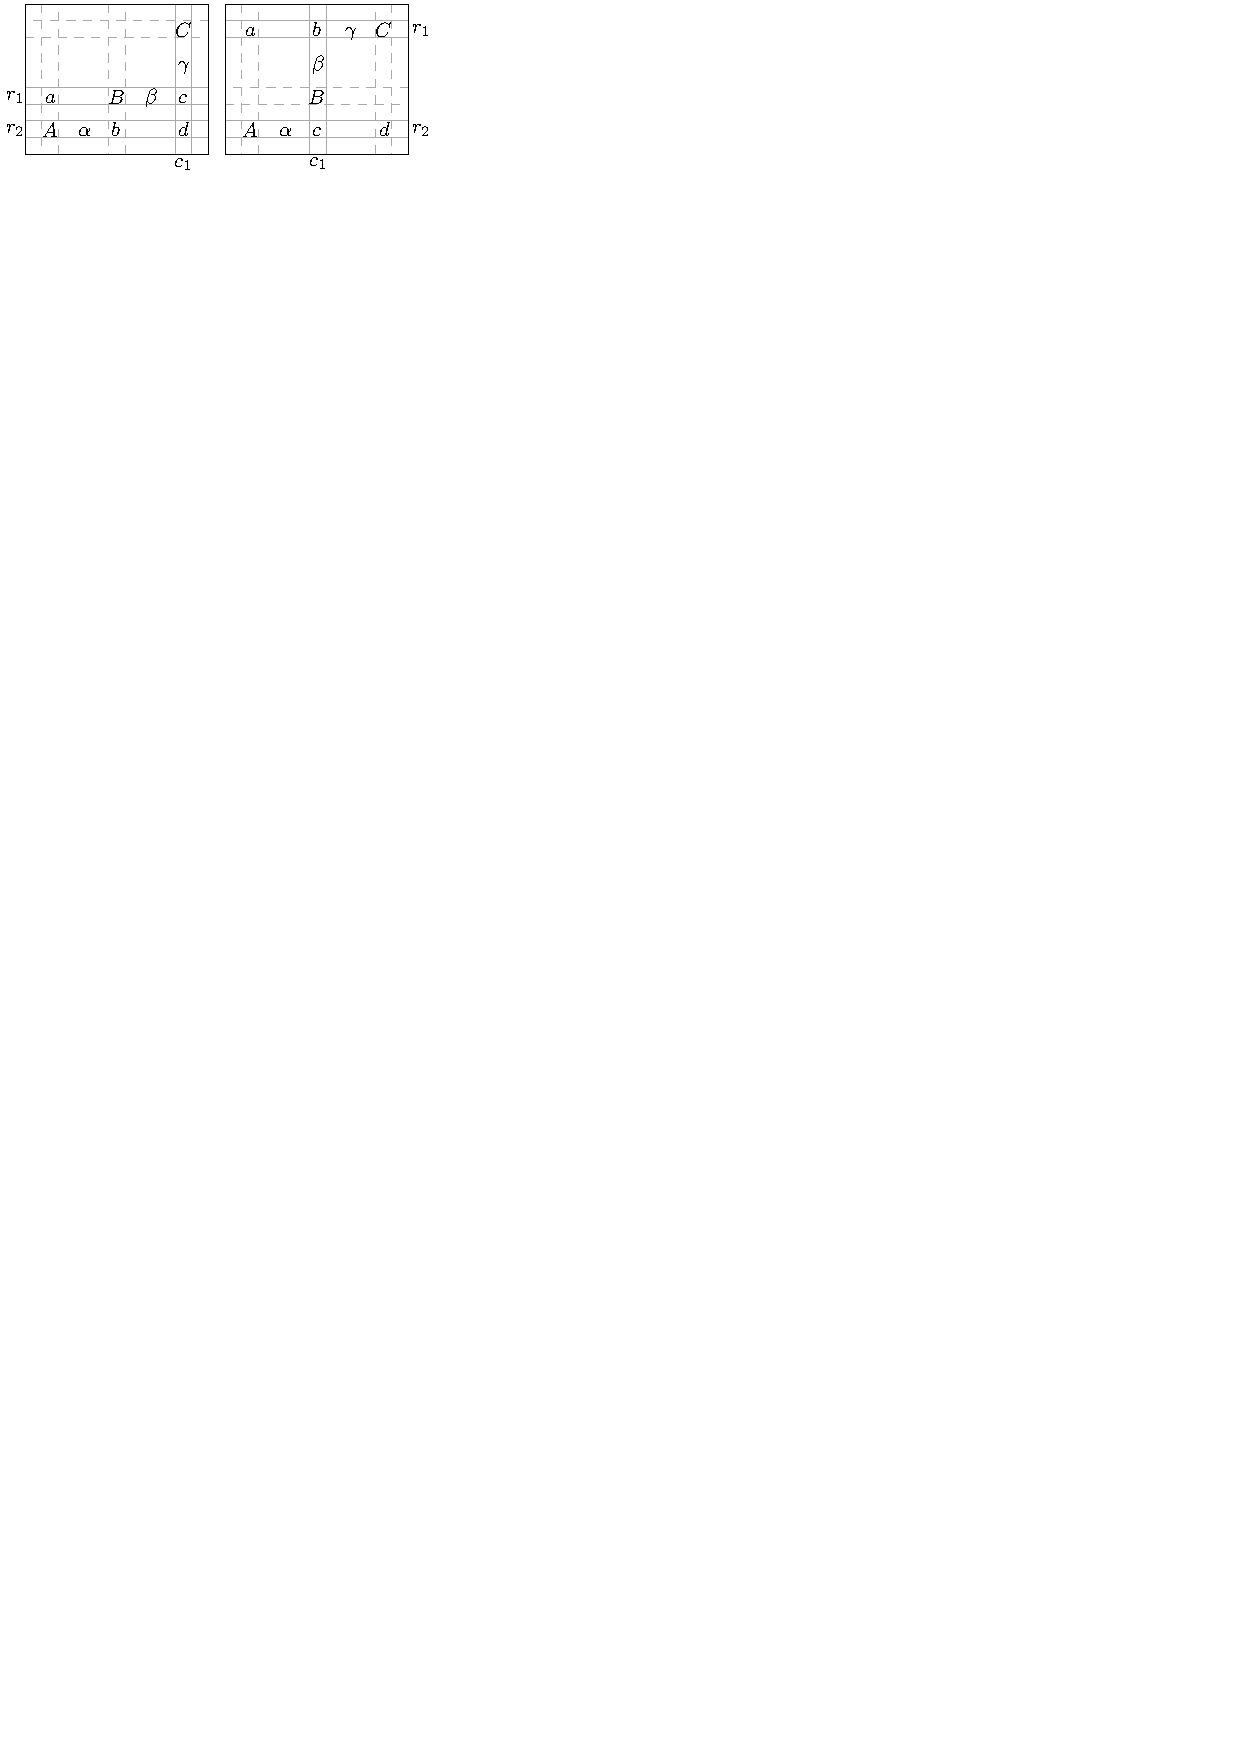
\includegraphics[width=120mm]{img/twoplusone.pdf}
	\caption{Structure of a pattern only having one-entries in two rows and one column that avoids all rotations of $P_1$.}
	\label{fig:twoplusone}
\end{figure}
\end{proof}

Combining all the lemmata we finally get the following result.

\begin{thm}
Let $P$ be a pattern avoiding all rotations of $P_1=\smm{ &\bullet& \\\bullet& & \\ & &\bullet}$, then $P$ is bounded. \qed
\end{thm}

\section{Chain rules}
In this section, we study what happens when we combine multiple classes that are bounded or unbounded.

\begin{thm}
\label{thm:boundunion}
Let $\mathcal{P}$ and $\mathcal{Q}$ be classes of patterns. If both $\mathcal{P}$ and $\mathcal{Q}$ are bounded then $Av(\mathcal{P}\cup\mathcal{Q})$ is bounded.
\end{thm}
\begin{proof}
We show $comp_{\mathcal{P}\cup\mathcal{Q}}\leq comp_\mathcal{P}+comp_\mathcal{Q}=C$.

For contradiction, let $M$ be a maximal matrix avoiding $\mathcal{P}\cup\mathcal{Q}$ having at least $C+1$ zero-intervals in a single row (or column). Without loss of generality it means there is more than $comp_\mathcal{P}$ zero-intervals usable for one-entries of the patterns from $\mathcal{P}$. Not let us change some zero-entries of $M$ to one-entries to get $M'\in Av(\mathcal{P})$. Clearly, it still contains more than $comp_\mathcal{P}$ zero-intervals usable for one-entries of the patterns from $\mathcal{P}$, which is a contradiction with the definition of $comp_\mathcal{P}$.

Similarly, the same inequality holds also for the column-complexity of $\mathcal{P}\cup\mathcal{Q}$ and so the union is bounded.
\end{proof}

Using induction, we can show that also a union of a finite number of bounded classes of finite sizes is bounded. Interestingly enough, unbounded classes are not closed the same way.

\begin{thm}
For every $1\leq i<j\leq4]$ is $\{P_i,P_j\}$ bounded.
\end{thm}
\begin{proof}
Due to symmetries it is enough to only consider $i=1$ and $j=[1,2]$.

\begin{itemize}
	\item $\{P_1,P_2\}$ is row-bounded: from Lemma~\ref{lemma:First} we have that one-entries $P_1[2,1],P_1[3,3],P_2[2,3]$ and $P_3[3,1]$ are row-bounded. For $P_1[1,2]$ and $P_2[1,2]$ we prove there are at most two zero-intervals usable for each of them. Otherwise, if there are three zero-intervals $z_1<z_2<z_3$ usable for $P_1[1,2]$ then the one-entries used to map $P_1[2,1]$ and $P_1[3,3]$ in a mapping created when a zero-entry of $z_1$ changes to one-entry used to map $P_1[1,2]$ together with a one-entry in between $z_2$ and $z_3$ give us a mapping of $P_2$ to $M$. Symmetrically, the same goes for $P_2[1,2]$ and $z'_3$.
	\item $\{P_1,P_2\}$ is column-bounded: from Lemma~\ref{lemma:First} combined with Observation~\ref{obs:transposebounded} we have that one-entries $P_1[1,2],P_1[3,3],P_2[1,2]$ and $P_3[3,1]$ are column-bounded. For $P_1[2,1]$ and $P_2[2,3]$ we prove there are at most two zero-intervals usable for each of them. Otherwise, if there are three zero-intervals $z_1<z_2<z_3$ (from top down) usable for $P_[2,1]$ then the one-entries used to map $P_1[1,2]$ and $P_1[3,3]$ in a mapping created when a zero-entry of $z_1$ changes to one-entry used to map $P_1[1,2]$ together with a one-entry in between $z_2$ and $z_3$ give us a mapping of $P_2$ to $M$. Symmetrically, the same goes for $P_2[2,3]$ and $z'_3$.
	\item $\{P_1,P_3\}$ is row-bounded: we can use the same proof as when showing that $\{P_1,P_2\}$ is column-bounded.
	\item $\{P_1,P_3\}$ is column-bounded: we can use the same proof as when showing that $\{P_1,P_2\}$ is row-bounded.
\end{itemize}
\end{proof}

We prove even stronger result by using a well known fact from the theory of ordered sets.

\begin{fct}[Higman's lemma]
\label{fct:Higman}
Let $A$ be a finite alphabet and $A^*$ be a set of finite sequences over $A$. Then $A^*$ is well quasi ordered with respect to the subsequence relation.
\end{fct}

\begin{thm}
$\sigma=Av\left(\smm{ &\bullet& \\\bullet& & \\ & &\bullet},\smm{ &\bullet& \\ & &\bullet\\\bullet& & },\smm{\bullet& & \\ & &\bullet\\ &\bullet& },\smm{ & &\bullet\\\bullet& & \\ &\bullet& }\right)$ is bounded. Moreover, every subclass is bounded.
\end{thm}
\begin{proof}
From Theorem~\ref{thm:boundedints} we know that elements of $\sigma$ fall into finitely many classes. For each we need to prove that it is bounded and also that it does not contain an infinite anti-chain. Knowing that we use Theorem~\ref{thm:boundunion} to obtain the result. Let us consider an $m$ by $n$ matrix $M\in\sigma$:
\begin{itemize}
	\item $M$ only contains up to three non-empty rows (columns):\\
		Clearly, if $M$ is maximal then it contains three rows made of one-entries and everything else is zero, so the number of one-intervals is bounded by three.\\
		
		We use words over alphabet~$A=\{a,b,c,d,e,f,g,h,i,j\}$ to describe each $M$ as follows. Let $r_1<r_2<r_3$ be the non-empty rows (if less then three are non-empty we choose extra values arbitrarily). We define $w_M\in A^*$ as follows. First, we use letter $g$ $r_1$ times, letter $h$ $r_2-r_1$ times, letter $i$ $r_3-r_2$ times and letter $j$ $m-r_3$ times to describe the number of rows of $M$. Then we describe columns from the first one to the last one as follows. For each 0 in $r_1$ we use letter $a$ and for 1, we use $ab$. For each 0 in $r_2$ we use letter $c$ and for 1, we use $cd$. For each 0 in $r_3$ we use letter $e$ and for 1, we use $ef$.
		
		If we have $w_M,w_{M'}\in A^*$ such that $w_M$ is a subsequence of $w_{M'}$ then we want to show that $M$ is an interval minor of $M'$. Let $r_1,r_2,r_3$ and $r_1',r_2',r_3'$ be the non-empty rows of $M$ and $M'$ respectively. Since the number of leading letters $g$ is not bigger in $w_M$, $M$ does not have more empty rows before $r_1$ than $M'$ does before $r_1'$ and similarly it has at most as many empty rows in between $r_1,r_2$ and $r_2,r_3$ and after $r_3$.

		Now consider there is $ab$ in $w_M$ and it corresponds to some $a\dots b$ in $w_{M'}$. We can always assume that in $w_{M'}$ the ``$a$'' is the one exactly before $b$. It can only happen that $abcdeface$ is a subsequence of $\textbf{ab}cea\textbf{cd}eac\textbf{eface}$ if the bold letters are used and since they correspond to one-entries lying in the following columns, this indeed corresponds to an interval minor (but it clearly does not have to mean that $M$ is a submatrix of $M'$).

		From Fact~\ref{fct:Higman} we have that $A^*$ is well ordered which means that matrices having at most three non-empty rows (columns) are well ordered (the construction can be extended to every fixed number of non-empty rows) and so they does not have an infitely long anti-chain.
	\item one-entries of $M$ lie in at most two rows and one column (or vice versa):\\
		The number of one-intervals of any such maximal $M$ is bounded by two.\\
		
		We use words over alphabet~$A=\{a,b,c,d,e,f,g\}$ and for non-empty rows~$r_1,r_2$ and column~$c_1$ we define $w_M$ as follows. We first encode each column in such a way that for each 0 in $r_1$ we use letter $a$ and for 1, we use $ab$. For each 0 in $r_2$ we use letter $c$ and for 1, we use $cd$. Right before and after the description of column $c_1$ we put letter $g$. Next we encode each row in such a way that for each 0 in $c_1$ we use letter $e$ and for each 1 letters $ef$. Right before and after the descriptions of rows $r_1$ and $r_2$ we again place letter $g$.
		
		Because of the distinct letters for encoding rows and columns we can apply the same analysis as we did in the previous case and since entries at $M[r_1,c_1]$ and $M[r_2,c_1]$ are separated from the rest by a special letter~$g$ there is no way to find a one-entry if it is not there.
	\item $M$ avoids $\smm{ &\bullet\\\bullet& }$ (or $\smm{\bullet& \\ &\bullet}$):\\
		From Theorem~\ref{thm:walking} we know $M$ is a walking matrix and any such maximal matrix only contains at most one one-intervals in each row and column.\\
		
		We use words over alphabet~$A=\{a,b,c,d\}$ and encode $M$ as follows. We choose an arbitrary walk of $M$ containing all one-entries and index its entries as $w_1\dots w_{m+n-1}$. Starting from $w_1$ we encode $w_i$ so that $a$ stands for 0 and $ab$ for 1 if $w_{i+1}$ lies in the same row as $w_i$ and we use $c$ for 0 and $cd$ for 1 if $w_{i+1}$ lies in the same column as $w_i$.
\end{itemize}

In the construction of words corresponding to matrices, we only made sure that $w_M\subseteq w_{M'}\Rightarrow M\im M'$ and the other impication does not hold. A different construction may lead to equivalence, but that is not necessary for our result.

We now use distinct alphabets to discribe different classes and when we given a potentialy infinite class of matrices from $\sigma$, we know that inside each class there is at most finite number of minimal matrices such that all of the rest contain a smaller one inside. Using induction on Theorem~\ref{thm:boundunion}, we have that each class is bounded and by applying induction with Theorem~\ref{thm:boundunion} once again we get that the union of the classes is also bounded.
\end{proof}

\begin{obs}
There exists a non-trivial bounded pattern~$P$ having an unbounded subset of $Av(P)$.
\end{obs}
\begin{proof}
Let $P=I_n$ (identity matrix) for $n>3$. From Lemma~\ref{lemma:walkpat} we have that $P$ is bounded. On the other hand, $Av(I_n,P_1)$ is unbounded, because the construction used in the proof of Theorem~\ref{thm:manyints} also works for this class.
\end{proof}

We define matrices to be bounded if they are both row-bounded and column-bounded. From what we proved so far, we see that a pattern $P$ is row-bounded if and only of it is column-bounded. But once we look at collections of patterns, this does not have to be true.

\begin{lemma}
There exists a class of patters~$\mathcal{P}$, which is row-bounded but column-unbounded.
\end{lemma}
\begin{proof}
Let $\mathcal{P}=\left\lbrace P=\smm{ &\bullet& \\\bullet& & \\ &\bullet& \\ & &\bullet},I_4=\smm{\bullet& & & \\ &\bullet& & \\ & &\bullet& \\ & & &\bullet}\right\rbrace$. We can use the same construction as we did in Theorem~\ref{thm:manyints}, just transposed, to prove $Av(\mathcal{P})$ is column-unbounded.

To prove that $\mathcal{P}$ is row-bounded, we take any $M$ maximal avoiding $\mathcal{P}$ and look at an arbitrary row. In Lemma~\ref{lemma:walkpat} we proved that patterns avoiding $\smm{ &\bullet\\\bullet& }$ are bounded and so every one-entry of $I_4$ is row-bounded. We need to proof the same for $P$. Using Lemma~\ref{lemma:First}, $P[2,1]$ and $P[4,3]$ are row-bounded. Using the first case of Lemma~\ref{lemma:I}, $P[3,2]$ is row-bounded. We prove that there are at most two zero-intervals usable for $P[1,2]$. For contradiction, let there be three -- $z_1<z_2<z_3$. It means there are at least two one-entries $e_1<e_2$ in between them. Now consider the partitioning of $P$ into $M$ when a zero-entry of $z_3$ is changed to one-entry used to map $P[1,2]$. Clearly, the one-entry used for mapping $P[2,1]$ lies under the left one-entry~$e$ bounding $z_3$ or in a latter column; otherwise we could use $e$ to map $P[1,2]$ and find the pattern in $M$. It may happen $e=e_2$, but still $e_1$ and the one-entries used for mapping $P[2,1],P[3,2]$ and $P[4,3]$ together give us a mapping of $I_4$ and so a contradiction with $M\in Av(\mathcal{P})$. It means that each one-entry of $P$ is also row-bounded and $Av(\mathcal{P})$ is row-bounded.
\end{proof}

Open questions:
\begin{itemize}
	\item $Av\left(\smm{ &\bullet& \\\bullet& & \\ & &\bullet},\smm{ &\bullet& \\ & &\bullet\\\bullet& & }\right)$ hereditary
\end{itemize}